%%%%%%%%%%%%%%%%%%%%%%%%%%%%%%%%%%%%%%%%%%%%%%%%%%%%%%%%%%%%%%%%%
%                            Info                               %
%%%%%%%%%%%%%%%%%%%%%%%%%%%%%%%%%%%%%%%%%%%%%%%%%%%%%%%%%%%%%%%%%
% This is the official SRL template for proposals and theses.

% The structure of the sections shown in this template
% demonstrate a typical proposal outline. Of course, you can
% adapt the structure to better suit your project.
% When writing a proposal, the declaration of originality is not
% necessary and can be removed.

% To customize the content of the title page and declaration of
% originality, make changes in the "Commands" section below. The
% title page and declaration are then automatically generated.

% The template is intentionally kept simple to keep it
% customizable and easy to use. Feel free to add any packages
% you need.

%%%%%%%%%%%%%%%%%%%%%%%%%%%%%%%%%%%%%%%%%%%%%%%%%%%%%%%%%%%%%%%%%
%                          Packages                             %
%%%%%%%%%%%%%%%%%%%%%%%%%%%%%%%%%%%%%%%%%%%%%%%%%%%%%%%%%%%%%%%%%
\documentclass[a4paper]{article}
\usepackage[utf8]{inputenc}
\usepackage[a4paper, top=3cm, bottom=3cm, left=3cm, right=3cm, marginparwidth=2cm, headsep=1.2cm]{geometry} % layout
\usepackage[bookmarks=true]{hyperref} % enables hyperlinks in the PDF
    \hypersetup{colorlinks=true, linkcolor=black, urlcolor=blue, citecolor=black} \urlstyle{same}
\usepackage{cleveref} \Crefformat{figure}{#2Fig.~#1#3} % makes referencing customizable (e.g. \Cref{}). See https://texblog.org/2013/05/06/cleveref-a-clever-way-to-reference-in-latex/)
\usepackage[nottoc, notlof, notlot]{tocbibind}  % includes bibliography in table of contents (TOC)

\usepackage[american]{babel}
\usepackage[sorting=none]{biblatex}
\DeclareLanguageMapping{american}{american-apa}
\addbibresource{bib.bib} % This defines where to take the references from. Currently the references are taken from the references.bib file. It is most convenient to use a reference manager (like Zotero or Mendeley) and link it to Overleaf. This way you can import and refresh your references with a few clicks (Import: New File -> From Zotero).
\usepackage{csquotes}
\usepackage{parskip}
\usepackage{todonotes}
\usepackage{booktabs}


\usepackage{graphicx} % required to include images
\usepackage{subfigure}
\usepackage{siunitx} % makes it easier to use units (e.g. \SI{15}{mm}). See: https://mirror.foobar.to/CTAN/macros/latex/contrib/siunitx/siunitx.pdf
\usepackage[font=small]{caption} % reduces the caption's font size
\usepackage{eso-pic} % required to add the titlepage background image
\usepackage{lipsum} % To generate lorem ipsum dummy text
\usepackage{pgfgantt} % For Gantt chart creation
\usepackage{fancyhdr} % Changes the header & footer style
\usepackage{bm}
\usepackage{lscape}
\usepackage{afterpage}
\usepackage{capt-of}

%%%%%%%%%%%%%%%%%%%%%%%%%%%%%%%%%%%%%%%%%%%%%%%%%%%%%%%%%%%%%%%%%
%                          Commands                             %
%%%%%%%%%%%%%%%%%%%%%%%%%%%%%%%%%%%%%%%%%%%%%%%%%%%%%%%%%%%%%%%%%
% Author
% Use \\ to separate multiple authors (e.g. Robert\\Nathalie\\Mike)
\newcommand{\myName}{Sebastiano Oliani}
\newcommand{\myEmail}{soliani@ethz.ch}
\newcommand{\myStudentID}{22-952-683}
\newcommand{\myLocation}{Zürich} % Only used for the signature in the declaration of originality

% Title
% Introduce line breaks with \\
\newcommand{\myTitle}{Learning a Policy for a Biomimetic Tendon-Driven Hand Combined with a Robotic Arm}

% Type of Thesis
% Use either "Semester Thesis", "Semester Thesis Proposal", "Master's Thesis" or "Master's Thesis Proposal"
\newcommand{\thesisType}{Semester Thesis}

% Date
% Use month + year only
\newcommand{\myDate}{11 January 2024}

% Supervisors
% Use \\ to separate multiple supervisors (e.g. Robert\\Nathalie\\Mike)
% Use full titles (e.g. Prof. Dr., Dr. )
\newcommand{\supervisors}{Yasunori Toshimitsu \\ Prof. Dr. Robert Katzschmann}

% Defines the command to set the title page background image (leave unchanged)
\newcommand\BackgroundPic{
    \put(0,0){
    \parbox[b][\paperheight]{\paperwidth}{%
    \vfill
    \centering
    \includegraphics[width=\paperwidth,height=\paperheight]{BackGroundPDF.pdf}
    \vfill
    }}}

% Header & Footer (leave unchanged)
\pagestyle{fancy}
\fancyhf{}
\rhead{
\includegraphics[height = 0.8cm]{template_figures/SRL_Logo.pdf}}
\lhead{
\includegraphics[height = 0.8cm]{template_figures/ETH_Logo.pdf}}
\fancyfoot[C]{\thepage}
\setlength{\headheight}{26.4pt}%
\renewcommand{\headrulewidth}{0.5pt}
\renewcommand{\footrulewidth}{0.5pt}
\definecolor{ETH-d-blue}{RGB}{56,92,155}
\definecolor{ETH-l-blue}{RGB}{205,214,230}

%%%%%%%%%%%%%%%%%%%%%%%%%%%%%%%%%%%%%%%%%%%%%%%%%%%%%%%%%%%%%%%%%
%                        Title Page                             %
%%%%%%%%%%%%%%%%%%%%%%%%%%%%%%%%%%%%%%%%%%%%%%%%%%%%%%%%%%%%%%%%%
% Don't change anything here
\begin{document}
\begin{titlepage}
\newgeometry{top=2cm, bottom=4cm, right=1.5cm, left=1cm}

\begin{center}
    \vspace*{6cm}
    \huge \textbf{\thesisType}\\
    \vspace*{0.75cm}
    \Huge \myTitle\\
    \vspace*{5cm}
    \huge \myName\\
    \vspace*{1.5cm}
    \LARGE \myDate\\
    \vfill
    Supervision\\
    \vspace*{0.5cm}
    \huge \supervisors 
\end{center}

\AddToShipoutPicture*{
\includegraphics[]{template_figures/titlepage_background.pdf}}
\end{titlepage}

%%%%%%%%%%%%%%%%%%%%%%%%%%%%%%%%%%%%%%%%%%%%%%%%%%%%%%%%%%%%%%%%%
%               Abstract & Table of Contents                    %
%%%%%%%%%%%%%%%%%%%%%%%%%%%%%%%%%%%%%%%%%%%%%%%%%%%%%%%%%%%%%%%%%
\pagenumbering{roman}

\begin{abstract}
    Dexterous Manipulation is an area of robotics in which multiple manipulators, or fingers, cooperate to grasp and manipulate objects. Biomimetic, dexterous robotic hands have the potential to replicate much of the tasks that a human can do, and to achieve status as a general manipulation platform. 
    
    Thanks to the recent advances in reinforcement learning (RL) combined with GPU-based highly parallelized simulations capable of simulating thousands of robots in parallel, RL-based controllers have become more scalable and approachable. Although simple tasks in industrial environments have already been solved by developing simple grippers, more complex tasks cannot be achieved without dexterous end-effectors. At the Soft Robotics Lab, the biomimetic tendon-driven Faive Hand has been developed to exploit reinforcement learning simulation environments and bring robotic hands into the real world.
    
    This work aims to enhance the current applications of the Faive hand by mounting it on a Franka Emika Panda arm, and using it to stack cubes on top of each other. Both the Faive Hand and the robotic arm are trained with reinforcement learning using the Nvidia Isaac Gym simulator. Thus, control policies are optimized by creating a simulation of the task and collecting data according to an episodic setting.
    
    After the reinforcement learning training reaches the desired behaviour, the control policies are implemented in a real physical environment. Objects in the scene are detected thanks to a perception system. As may happen when testing policies that have been trained using an episodic setting, many issues are encountered in closing the sim-to-real gap. Even if some individual components of the entire control pipeline are separately working, the task is not fully achieved in the end.
\end{abstract}

\newpage
\section*{\textit{Summary of notation}}
\vspace{1cm}
\begin{tabular}{p{2cm} p{8cm}}
    $\bm q_{arm}$ & Generalized joint arm coordinates\\
    $\bm q_{hand}$ & Generalized joint hand coordinates\\
    $\bm q_{max}$ & Generalized coordinates upper limit\\
    $\bm q_{min}$ & Generalized coordinates lower limit\\
    $\bm q_{start}$ & Generalized coordinates initial condition\\
    $\bm p_{grab}$ & Position of the grabbing cube\\
    $\bm p_{ref}$ & Position of the reference cube\\
    $\bm p_{hand}$ & Position of the hand's palm\\
    $\bm p_{fingertip}$ & Position of the hand's fingertips\\
    $\bm p_{x}$ & Position X-coordinate\\
    $\bm p_{y}$ & Position Y-coordinate\\
    $\bm p_{z}$ & Position Z-coordinate\\
    $\hat{\bm j}$ & Y-coordinate unit vector\\
    $\hat{\bm k}$ & Z-coordinate unit vector\\
    $\bm l_{grab}$ & Length of the grabbing cube\\
    $\bm a$ & Actions\\
    $\mathcal{N}(\mu, \sigma^2)$ & Normal distribution with mean $\mu$ and variance $\sigma^2$\\
    $\mathcal{U}(a, b)$ & Uniform distribution within $a$ and $b$\\
\end{tabular}


\newpage
\tableofcontents
\newpage

\pagenumbering{arabic}

%%%%%%%%%%%%%%%%%%%%%%%%%%%%%%%%%%%%%%%%%%%%%%%%%%%%%%%%%%%%%%%%%
%                      Document Start                           %
%%%%%%%%%%%%%%%%%%%%%%%%%%%%%%%%%%%%%%%%%%%%%%%%%%%%%%%%%%%%%%%%%

\newpage

\section{Introduction}

\subsection{Motivation}
In industry, robotic assembly methods may achieve high precision, accuracy, and reliability. However, these methods can be highly restrictive. They often use expensive equipment, require custom fixtures, have high setup times (e.g., tooling design, waypoint definition, parameter tuning) and cycle times, and are sensitive to variation (e.g., part appearance, location). Custom tooling and part-specific engineering are also cost-prohibitive for high-mix, low-volume settings.
In the last decades, physics simulation has become a powerful tool for robotics development. Simulators have primarily been used to verify and validate robot designs and algorithms. Recent research has demonstrated a host of other applications: creating training environments for virtual robots, generating large-scale grasping datasets, inferring real-world material parameters, simulating tactile sensors, and training RL agents for manipulation and locomotion. Compelling works have now shown that RL policies trained in simulation can be transferred to the real world \cite{narang2022factory}.

Dexterous manipulation is one of the hottest topics of research these days. 
% Dexterous manipulation differs from traditional robotics primarily in that the manipulation is object-centered. That is, the problem is formulated in terms of the object to be manipulated, how it should behave, and what forces should be exerted on it. % 
Dexterous manipulation, requiring precise control of forces and motions, cannot be accomplished with a conventional robotic gripper; fingers or specialized robotic hands must be used \cite{844067}. Although some simple tasks in the industrial environment have been solved, the need for robots that can help humans in some unstructured environments such as the domestic environment (e.g., helping blind people with daily routines) and some dangerous environments (e.g., nuclear decommissioning) is significant. When facing a complex unstructured environment, one robot needs to deal with a lot of tasks and, ideally, one robot needs to carry different end-effectors for different tasks, which is unpractical. Hence, the ability to operate with the dexterity of the robot is necessary \cite{10.3389/fnbot.2022.861825}.

\subsection{State-of-the-Art}
Over the past decades, many dexterous multi-fingered hands have been designed. In 1984, the Center for Engineering Design at the University of Utah, and the Artificial Intelligence Laboratory at the Massachusetts Institute of Technology designed the UTAH/MIT hand with three fingers and a thumb aiming at machine dexterity \cite{JacobsenIKJB86}, and later HIT developed the DLR/HIT Hand II \cite{Liu2008MultisensoryFD}. Also, there are some commercial products such as the Shadow Hand \cite{article} and the Allegro hand\footnote{Website: \url{http://wiki.wonikrobotics.com/AllegroHandWiki/index.php/Allegro_Hand_v4.0}} (see Figure \ref{fig:foobar}).
Apart from the dexterous humanoid robotic hands, some simpler robotic manipulators with fewer fingers and lower degrees of freedom (DoF) have been designed for better robustness and lower price. The current applications of robotic hands in the factories still use traditional engineering and analysis techniques. Typically, some robots with simple end-effectors are widely used in the manufacturing industry for packaging and palletizing. Similarly, agricultural robotic hands with several end-effectors and painting robotics are good examples of the application of robotic hands in the structured industry environment \cite{10.3389/fnbot.2022.861825}.

\begin{figure}[!hb]
    \centering
    \subfigure[]{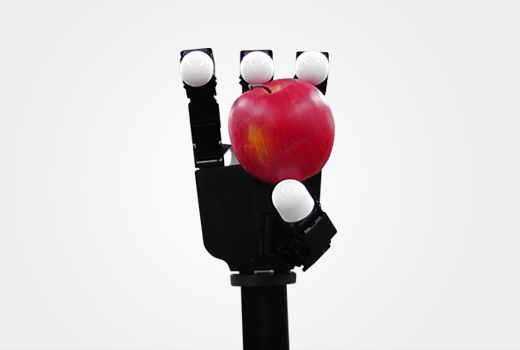
\includegraphics[width=0.25\textwidth]{images/0.ou7zie56oafig3.png}} 
    \subfigure[]{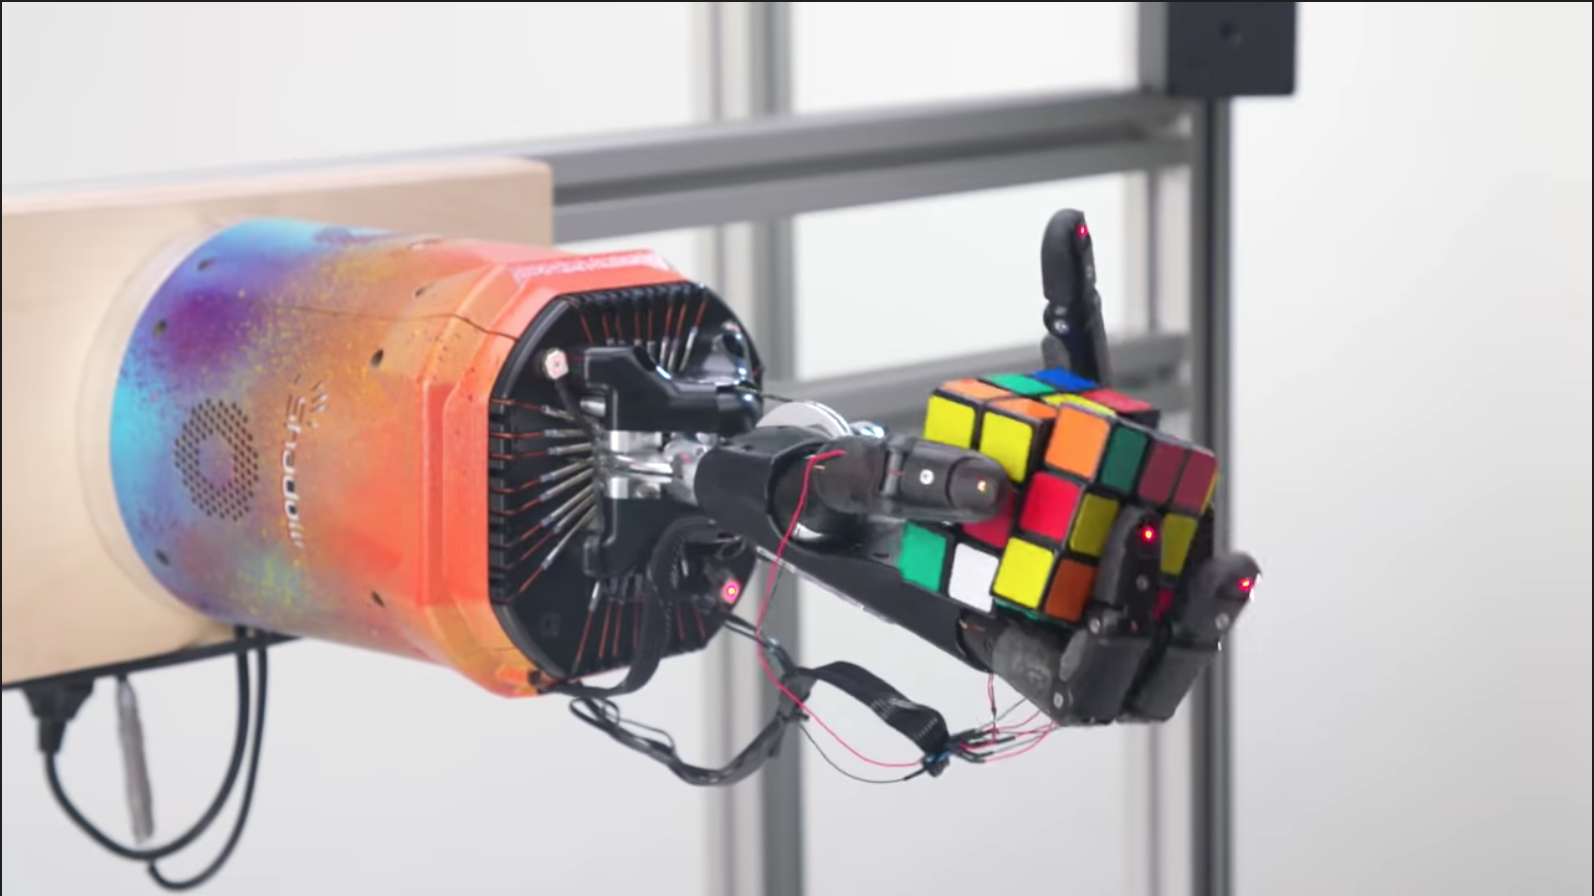
\includegraphics[width=0.30\textwidth]{images/OpenAI Rubiks Cube.png}} 
    \subfigure[]{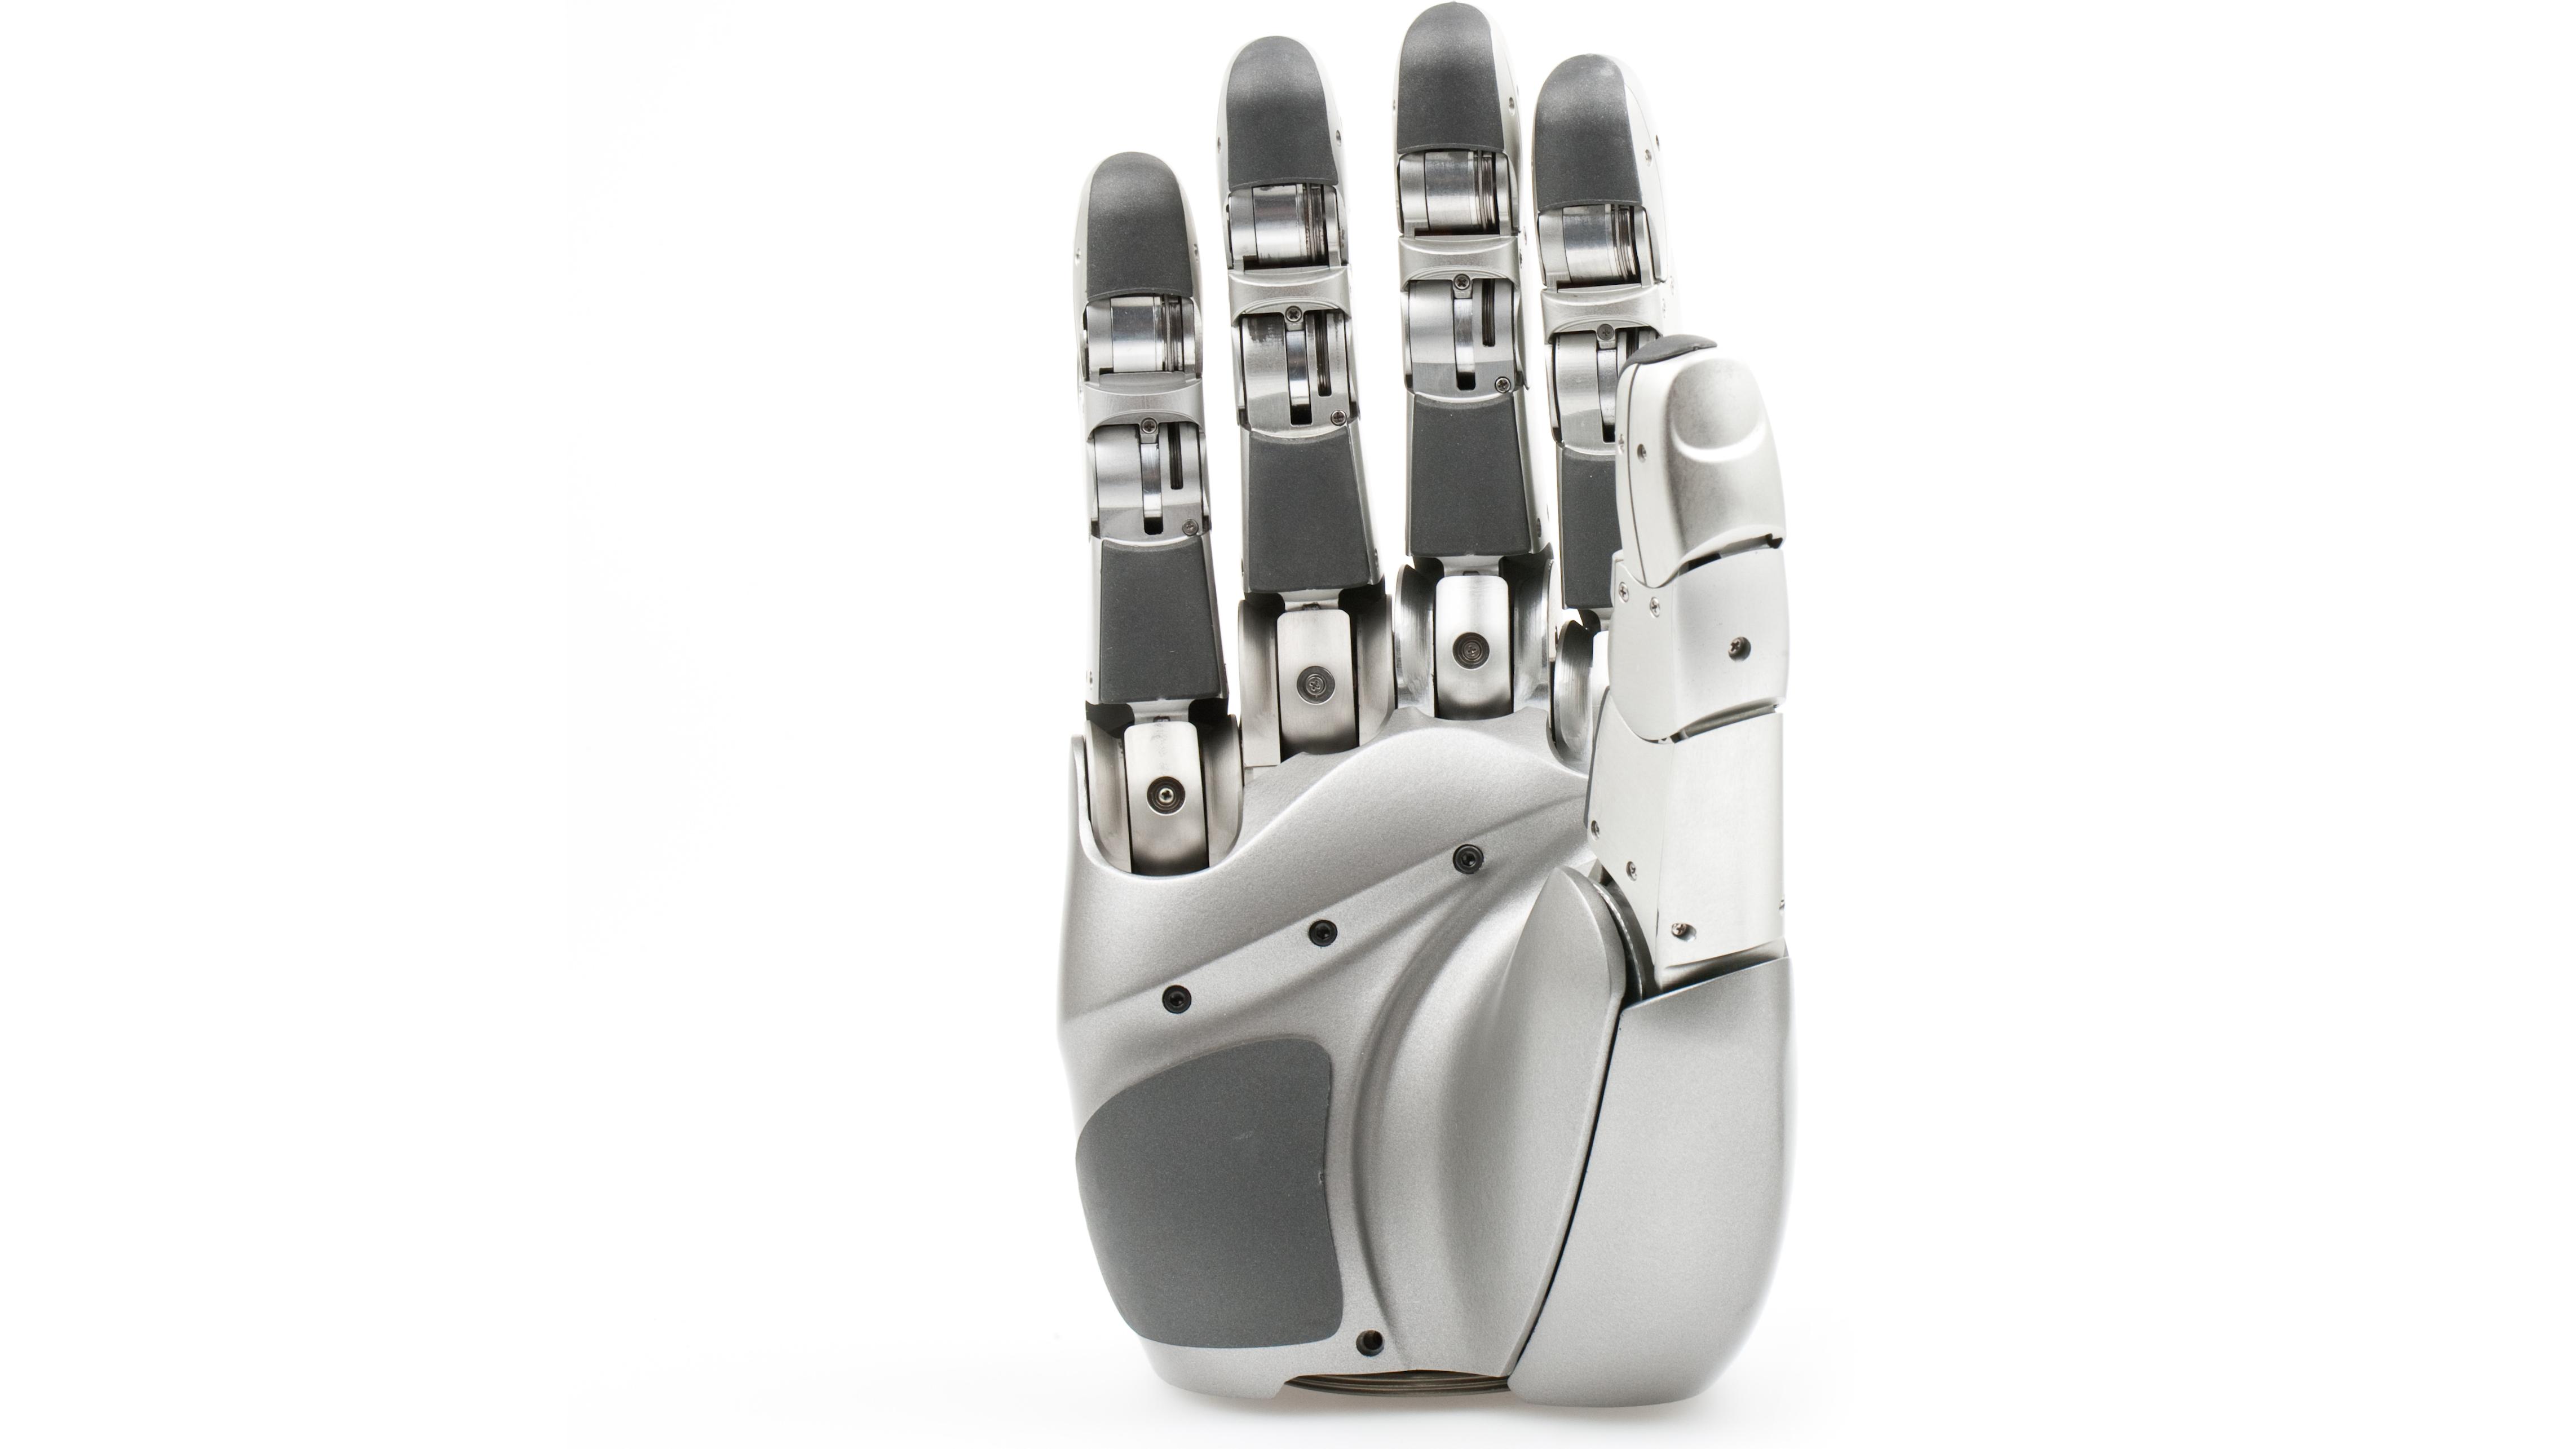
\includegraphics[width=0.30\textwidth]{images/ffh_2010_stehend_freigestellt_4569x2570_orig.jpg}}
    \caption{(a) Allegro Hand (b) Shadow Hand (c) DLR Hand II }
    \label{fig:foobar}
\end{figure}

Although the mechanical design of smart manipulators has improved greatly, the actual dexterity of the robotic hands is far inferior to that of the human hand. On one hand, lots of sensors and actuators of the human hand make it almost impossible to design a robotic hand which is similar to the human hand, and on the other hand, the control of the robotic hand to realize dexterous manipulation is still an urgent problem to solve. Model-based approaches fail in real applications due to inaccuracies in the models, and because algorithms must change as the object or the manipulator changes. In contrast, reinforcement learning is more suitable for dealing with the sequential decision problem.
Therefore, the combination of deep learning and reinforcement learning called deep reinforcement learning is proposed to realize more complicated problems involving perception and decision-making. However, the application of deep reinforcement learning to dexterous manipulation has some disadvantages. First, the sparse reward makes the training hard, and for complex tasks, it is time-consuming and the requirement of computing power is high. Furthermore, deep reinforcement learning requires many samples obtained by trial and error, which are nearly unavailable in a robotic system. To solve this problem, besides the improvement of the reinforcement learning algorithm, two solutions are usually considered: learning from demonstration and transferring the policy learned in simulation to reality. These two approaches will greatly enhance the efficiency of the algorithm.

Another key element when working with reinforcement learning is the sim-to-real gap. This term describes the discrepancies between simulation and real robots that make the transformation challenging. Transforming the policy directly to the real world may cause various consequences, the lesser of which is a decline in success and the more serious of which is the instability of the system that may destroy the robotic hands or the environment. Hence, closing the sim-to-real gap is the main issue when mentioning the sim-to-real problem. The sim-to-real problem is not unique to the field of reinforcement learning or dexterous manipulation, but a general problem in machine learning for robotics. The main approach widely used for closing the sim-to-real gap is domain randomization. The main idea of domain randomization is to randomize the simulation with disturbance, i.e. variations in the values of the main parameters of the simulation like friction coefficients, mass, contact model, etc. Through exposure to various environments, the agent trained in simulation can adapt to a wide range of environments, and, in the end, succeed in closing the sim-to-real gap.

The implementation of reinforcement learning algorithms using robotic arms combined with human-like hands is a very active research topic. In those cases, imitation learning is adopted to improve the training and transfer the learned policy into the real environment. If imitation learning is not implemented, then mostly standard-grippers are used \cite{breyer2019comparing}. Common tasks covered in nowadays research are opening a drawer, opening a door, picking up a ball, in-hand rotation, etc.
    
\subsection{Current set-up developed at Soft Robotics Lab}

\begin{figure}[!hb]
    \centering
    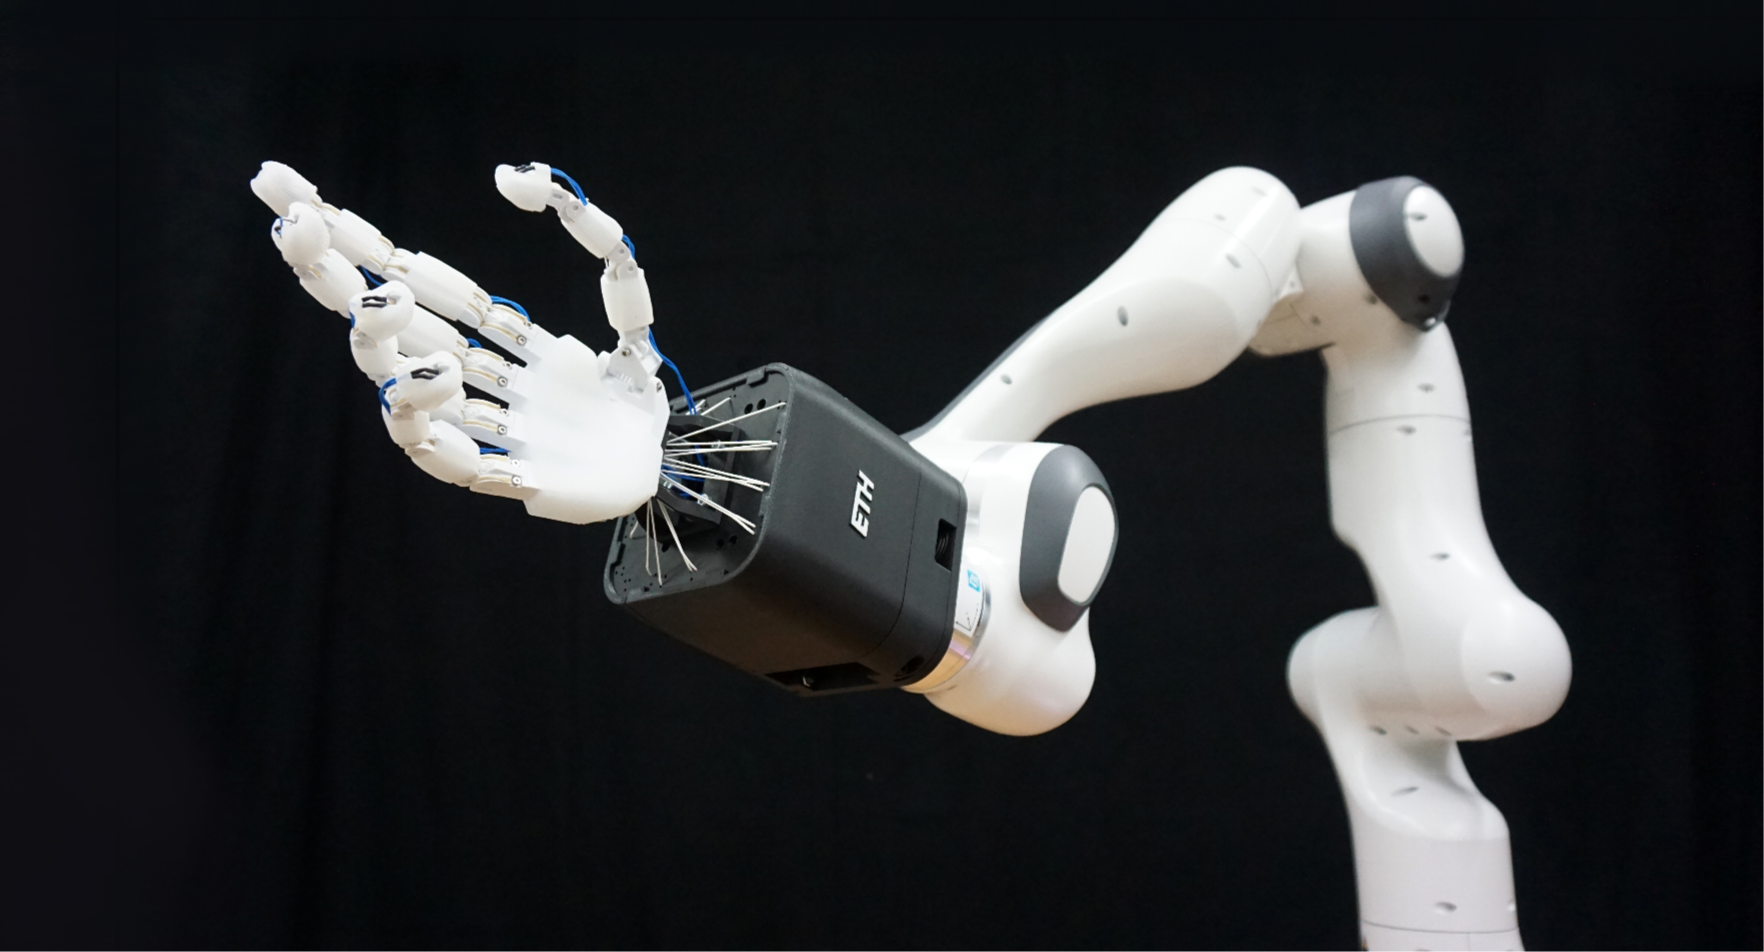
\includegraphics[scale=0.2]{images/4a78b0_c2490c2428ba4e19bf12687e84801176~mv2.png}
    \caption{Franka Emika and Faive Hand Proto0.}
\end{figure}

The Faive Hand has been developed at the Soft Robotics Lab. It is a biomimetic dexterous tendon-driven robotic platform for exploring dexterous manipulation. The so-called Proto0-version of the hand uses 3D-printed components and servo motors for accessible and simple manufacturing. However, in addition to the challenges inherent to controlling a high-DoF robotic hand for manipulation, this hand has features that do not exist in other dexterous hands trained with reinforcement learning, such as rolling contact joints that rotate without a fixed axis of rotation. The hand currently does not have internal joint angle encoders, but the joint angles must be estimated from the tendon length, which can be calculated from the servo motor angles.

The Faive Hand contains 11 actuatable degrees of freedom, three in the thumb and two for each of the other fingers. Each finger contains a coupled joint at the distal end, and thus there are 16 joints in total.
All of the joints are implemented as rolling contact joints, except for two hinge joints mounted in the thumb. These rolling joints are composed of two articulating bodies with adjacent curved contact surfaces connected by a pair of crosswise ligament strings. They have advantages such as impact compliance, low friction or greater range of motion \cite{toshimitsu2023getting}.

These features were implemented in the simulation framework. Then the Faive Hand was simulated in Nvidia Isaac Gym to run a closed-loop RL-trained policy (see Figure \ref{FH}). The first task that was chosen with the given set-up was the in-hand rotation of a sphere in a target direction.

The policy is trained with reinforcement learning with advantage actor-critic (A2C) using asymmetric observations (where different sets of observations are given to the actor and critic). The PPO algorithm \cite{schulman2017proximal} with the implementation from the open-source repository \textit{rl games}\footnote{D. Makoviichuk and V. Makoviychuk, “rl-games: A high-performance framework for reinforcement learning,” \url{https://github.com/Denys88/rlgames}, May 2021.} is adopted. MLP networks are used as actor and critic.

\begin{figure}[!hb]
    \centering
    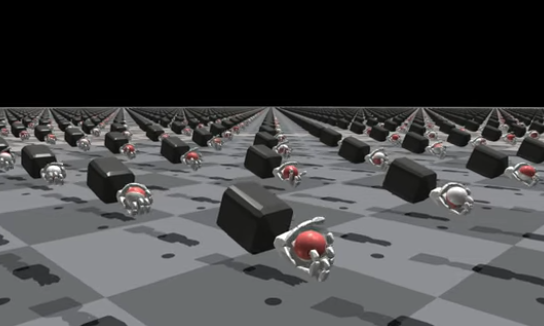
\includegraphics[scale=0.7]{images/Screenshot from 2023-10-11 23-38-03.png}
    \caption{Faive Hand training in Isaac Gym.}
    \label{FH}
\end{figure}

As part of the set-up, the Faive Hand is mounted on a Franka Emika Panda arm\footnote{Website: \url{https://www.franka.de/} (see Figure \label{FEP}), and datasheet: \url{https://www.phytronrobotics.com/files/136589731.pdf}}. This industrial robot arm has seven degrees of freedom, 18 kg weight and a 3 kg payload. It originally mounts a two-finger gripper, but, to develop the Semester Thesis, the original gripper will be substituted by the Faive Hand.

\newpage

\begin{figure}[!hb]
    \centering
    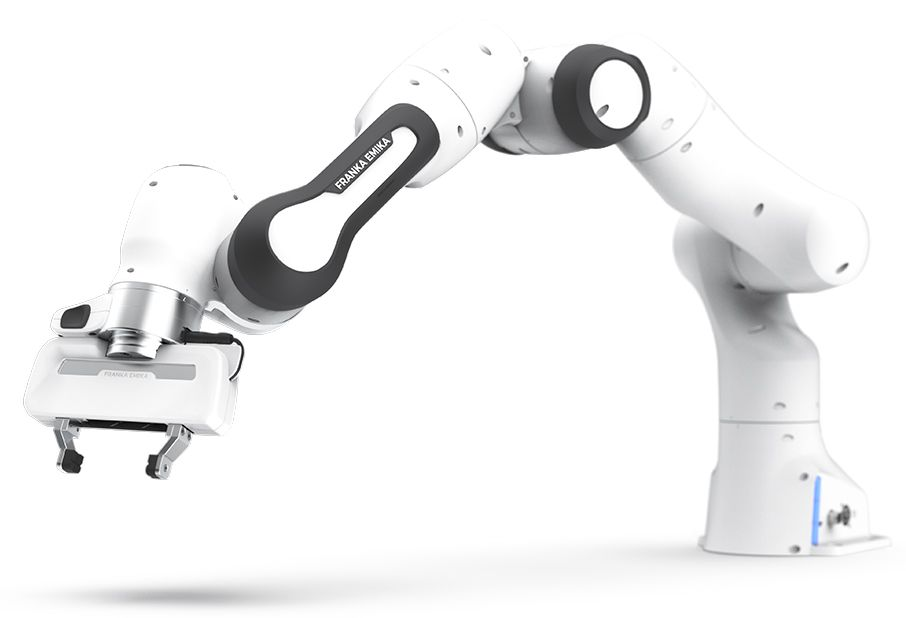
\includegraphics[scale=0.3]{images/1619174709718.jpg}
    \caption{Franka Emika Panda with its standard two-finger gripper.}
    \label{FEP}
\end{figure}

This work uses a new version of the Faive Hand, called Proto2-version (see Figure \ref{P2}). This newer version uses rolling contact joints only, even for the thumb. It gains the ability to perform abduction movements with the finger and it revises the thumb anatomy to match the human hand better. This new version consists of 16 actuatable degrees of freedom, four in the thumb and three in the other fingers.

\begin{figure}[!hb]
    \centering
    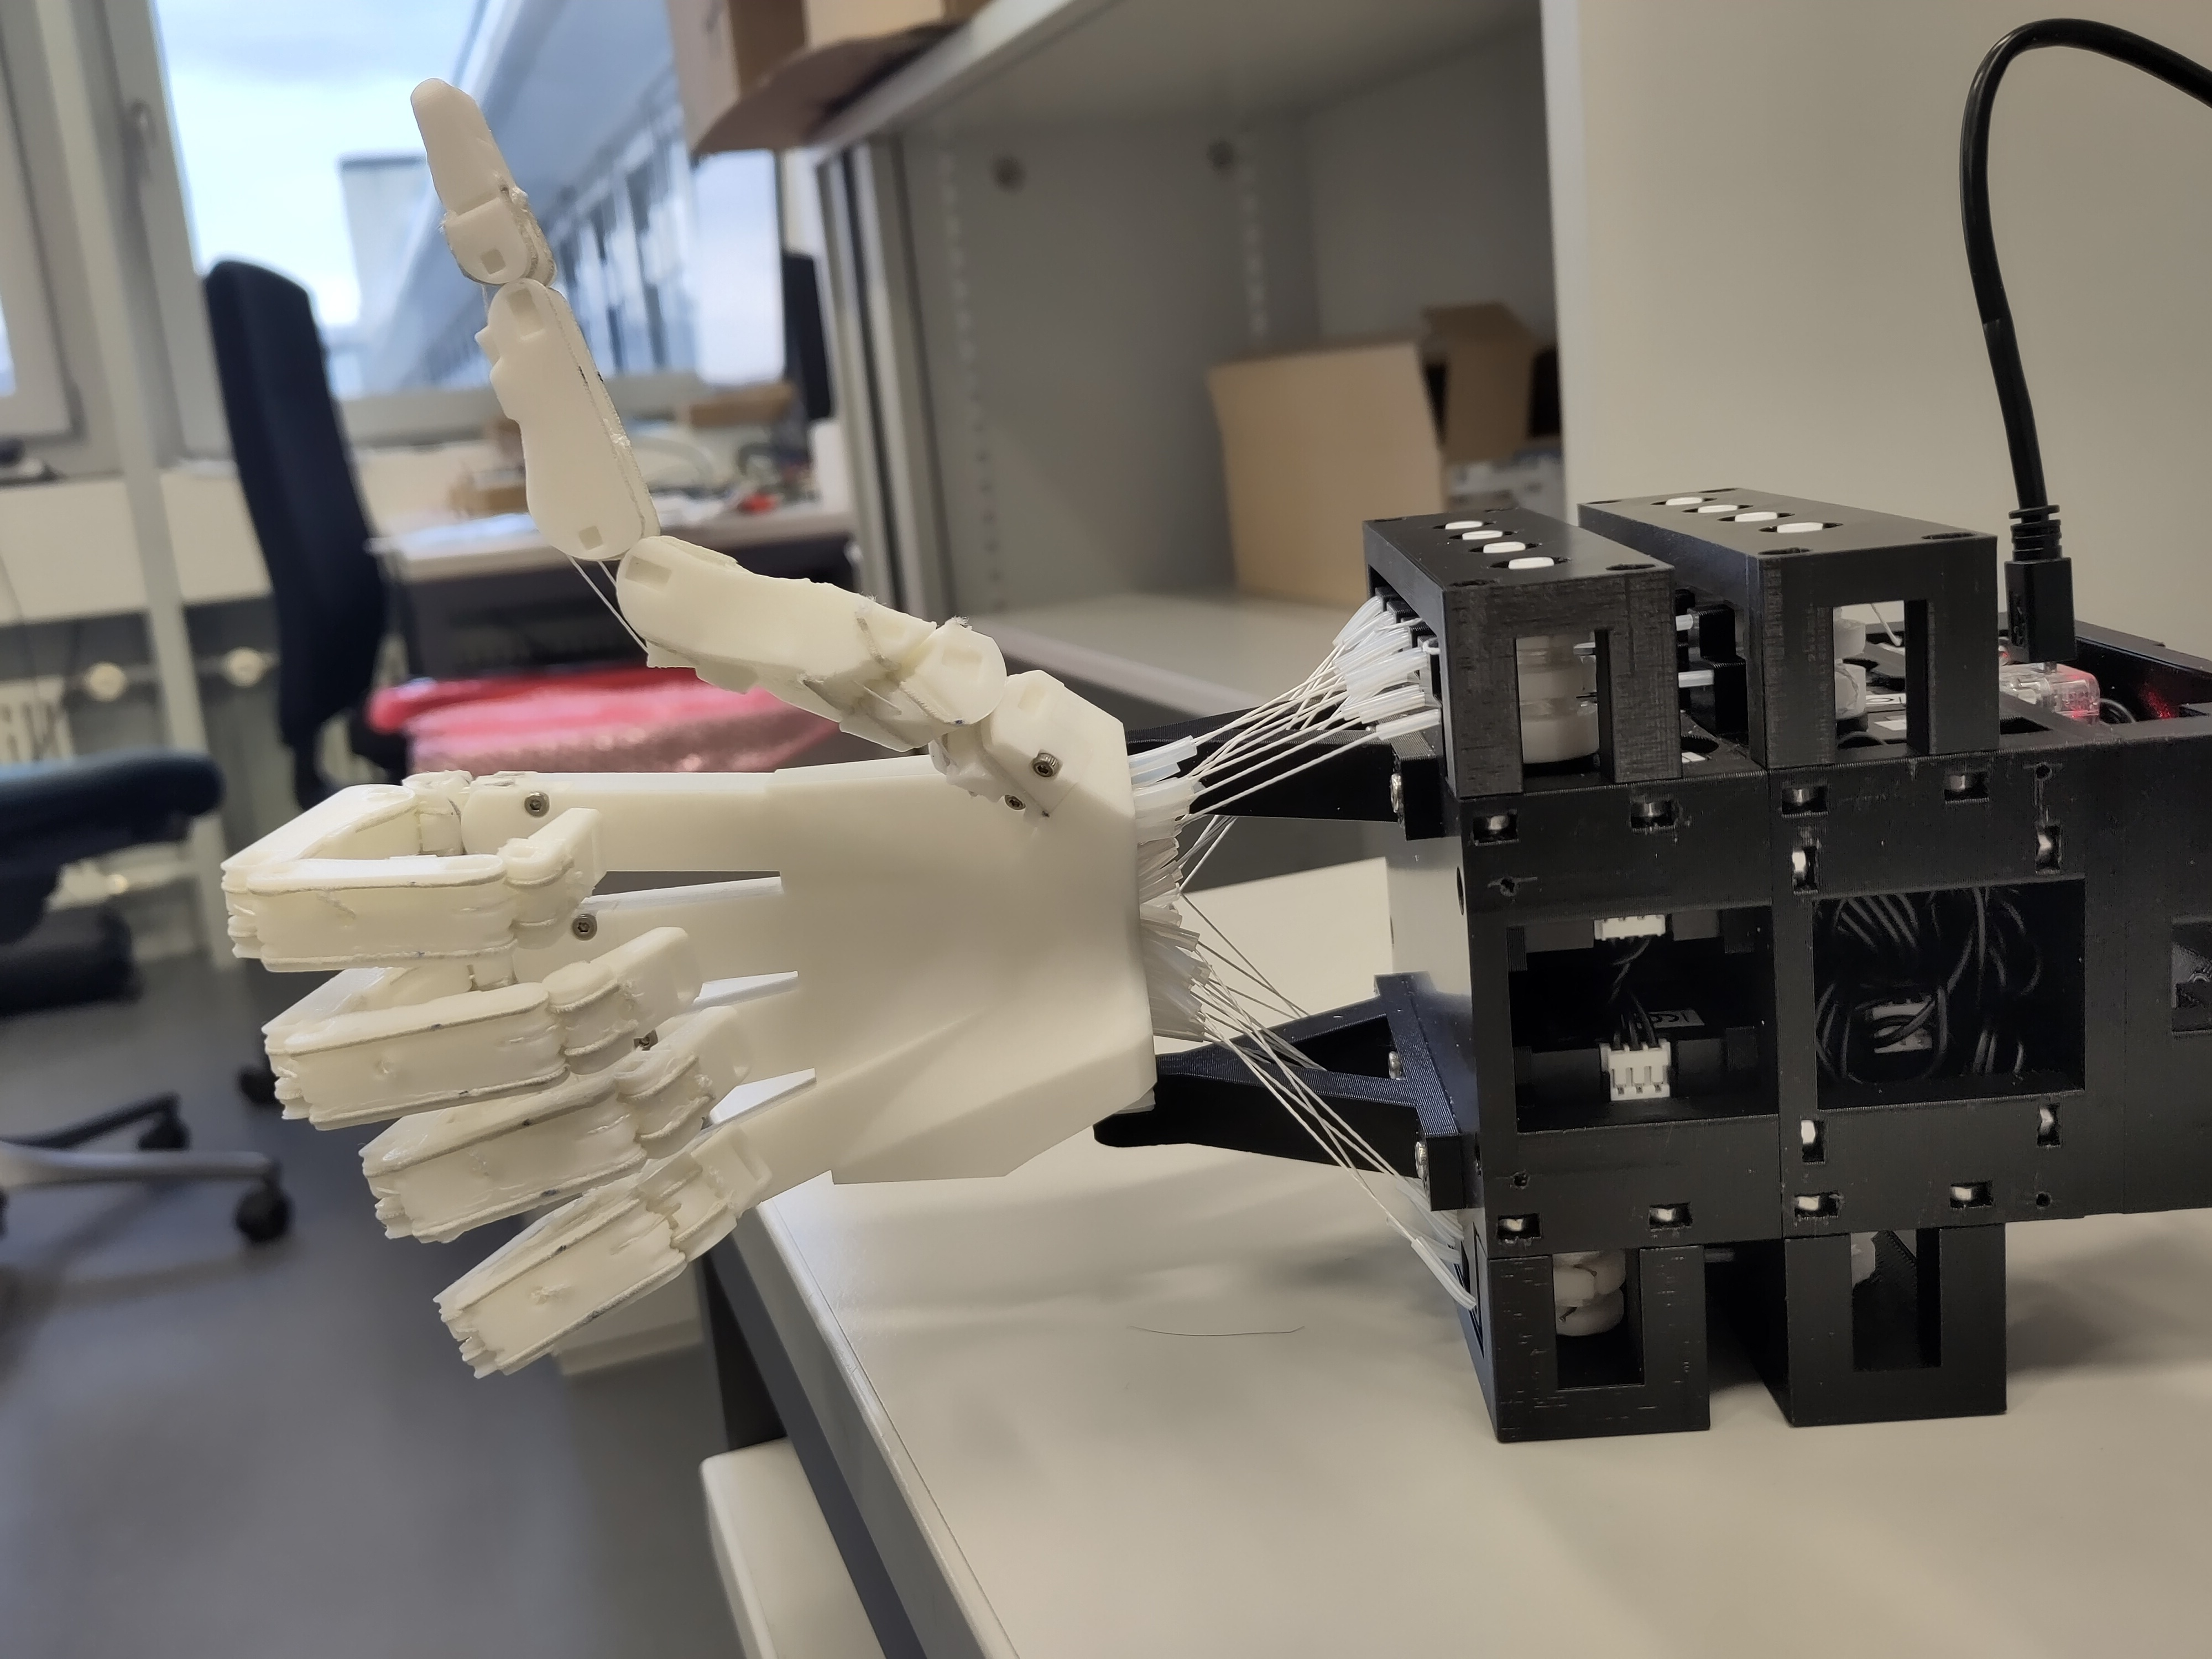
\includegraphics[scale=0.07]{images/IMG_20230327_190549.jpg}
    \caption{Faive Hand Proto2.}
    \label{P2}
\end{figure}


\newpage 

\section{Background}% previously: Work packages
As robotics hardware becomes more complex and capable, the importance of simulation tools increases. Simulators play a key role in training robots, improving the learning process's safety and iteration speed through hardware accelerators. Training inside simulators offers an efficient and scalable platform via trial and error with no safety issues observed in the real world. MuJoCo\footnote{\url{https://mujoco.org/}}, owned by Google DeepMind, and Isaac Gym\footnote{\url{https://developer.nvidia.com/isaac-gym}}, owned by Nvidia, are exploited to develop this Semester's Thesis.

%%%%%%%%%%%%%%%%%%%%%%%%
%       MuJoCo         %
%%%%%%%%%%%%%%%%%%%%%%%%
\subsection{MuJoCo}

    The name MuJoCo stands for Multi-Joint dynamics with Contact \cite{6386109}. It represents the state in joint coordinates and simulates contacts using the Linear Complementary Problem (LCP). It has several unique features which are rarely needed for simulation purposes but greatly facilitate control applications:
    \begin{itemize}
        \item Models are created in XML format and then compiled automatically into low-level data structures optimized for runtime computation.
        \item The same dynamical system can be evaluated in parallel for different states and controls. This is useful for approximating derivatives via finite differencing, which enables numerical optimization.
        \item Inverse dynamics can always be computed even in the presence of contacts and equality constraints.
        \item Actuator dynamics such as the pressures inside pneumatic or hydraulic cylinders as well as the activations of biological muscles can be modeled. Actuators can transmit forces via linkages or tendons too.
    \end{itemize}

\begin{figure}[!hb]
    \centering
    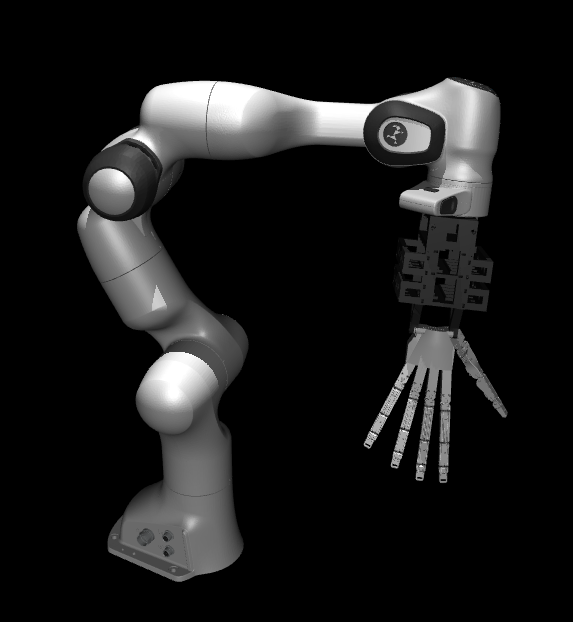
\includegraphics[scale=0.45]{images/Screenshot from 2023-10-15 20-21-24.png}
    \caption{Franka Emika and Faive Hand Proto2 visualized in Mujoco.}
    \label{FPFH}
\end{figure}

\newpage
%%%%%%%%%%%%%%%%%%%%%%%%
%      Isaac Gym       %
%%%%%%%%%%%%%%%%%%%%%%%%
\subsection{Isaac Gym}
  
    Isaac Gym allows training policies for a wide variety of robotics tasks using GPU (see Figure \ref{Some IG}). Both physics simulation and the neural network policy training reside on GPU and PyTorch tensors\footnote{\url{https://pytorch.org/}}. This leads to fast training times for complex robotics tasks on a single GPU with 2-3 orders of magnitude improvements compared to conventional reinforcement learning training that uses a CPU-based simulator and GPU for neural networks \cite{makoviychuk2021isaac}.
    
    Through Isaac Gym, it is possible to create and populate a scene with robots and objects, supporting loading data from the common URDF and MJCF file formats. Each environment can be duplicated many times in different instances, and Isaac Gym allows varying parameters between them, e.g. via Domain Randomization.
    
    Environments are simulated simultaneously in parallel without interaction with other environments. Isaac Gym also includes a basic Proximal Policy Optimization (PPO) implementation and a straightforward reinforcement learning task system.

\begin{figure}[!hb]
    \centering
    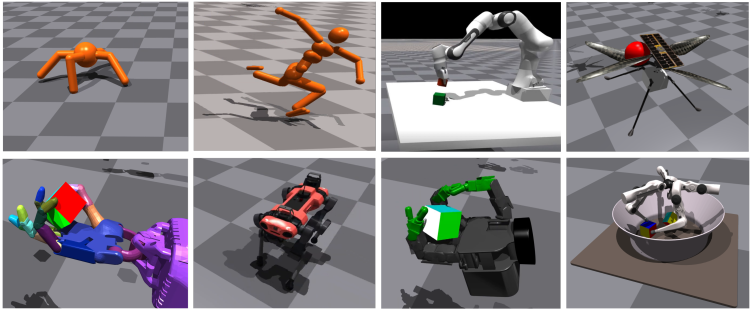
\includegraphics[scale=0.5]{images/Screenshot from 2023-10-10 13-20-57.png}
    \caption{Isaac Gym allows high-performance training in a variety of robotics environments. Top: Ant, Humanoid, Franka-cube-stack, Ingenuity. Bottom: Shadow Hand, ANYmal, Allegro, TriFinger.}
    \label{Some IG}
\end{figure}

%% ROS was here

\newpage

\section{Methodology}
This Semester’s Thesis has been pursued from the beginning of September 2023 to the beginning of January 2024. This section describes the task to implement, the approach, the results of the simulations, the implementation set-up and the final experiment results.

\subsection{Task selection}

In \cite{toshimitsu2023getting}, the Faive Hand Proto-0 has been trained in Nvidia Isaac Gym to rotate a ball along the y-axis. To enhance the possible applications, the following Semester Thesis wants to implement a reinforcement learning algorithm to stack cubes on top of each other in a real environment using the Faive Hand as the end-effector of the robotic arm. The entire system composed of Franka Emika Panda and Faive Hand is trained in simulation to obtain a Reinforcement Learning policy. The main goal is to obtain a working policy by only using the results coming from the simulation. Therefore, more advanced methods as imitation learning that exploits human demonstrations are not used. A similar task is already available as an example in Nvidia IsaacGymEnvs (see Figure \ref{FCS}) and its implementation can be found on \href{https://github.com/NVIDIA-Omniverse/IsaacGymEnvs/blob/main/isaacgymenvs/tasks/franka_cube_stack.py}{GitHub}\footnote{\url{https://github.com/NVIDIA-Omniverse/IsaacGymEnvs/blob/main/isaacgymenvs/tasks/franka_cube_stack.py}}. Its rewards, observations and control law were considered as an initial reference in the implementation of this Semester's Thesis.

\begin{figure}[!hb]
    \centering
    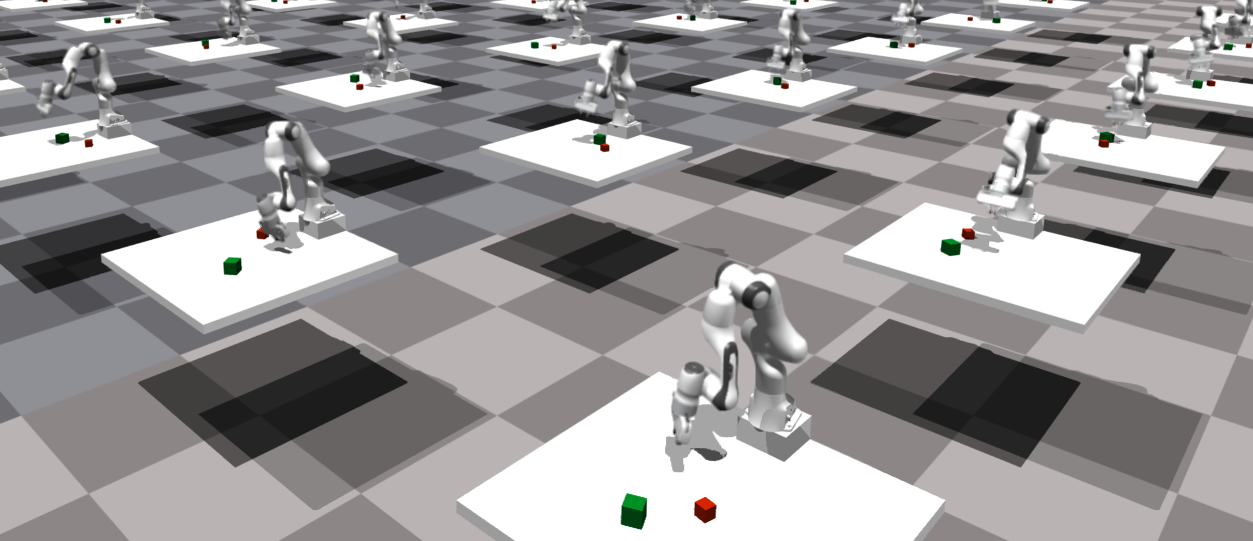
\includegraphics[scale=0.3]{images/Screenshot from 2023-10-15 20-32-34.png}
    \caption{Franka-Cube-Stack implementation from Nvidia IsaacGymEnvs.}
    \label{FCS}
\end{figure}

\subsection{Approach}

\subsubsection{Simulation environment}

First of all, a 3D model of the robotic arm combined with the Faive Hand is created using MuJoCo (see Figure \ref{FPFH}). In particular, the 3D model of the robotic arm is open-source, and can be found in the \href{https://github.com/google-deepmind/mujoco_menagerie/tree/main/franka_emika_panda}{MuJoCo Menagerie}, a collection of high-quality models curated by Google DeepMind and published on GitHub. Then, similarly to what was done in \cite{toshimitsu2023getting}, the GPU-based simulator Nvidia Isaac Gym is used to simulate the robot for training the policy. 4096 environments are simulated in parallel on a single NVIDIA A10G GPU. The simulation is run at 60 Hz, while the policy runs every three steps, resulting in a 20 Hz policy.
The data are collected using Weights \& Biases\footnote{\url{https://wandb.ai/site}} while running the training in Nvidia Isaac Gym (see Figure \ref{IG}). In this way, it is possible to collect short videos of the agent's behaviour, and plot quantities of interests, like rewards or observations, that can be further exploited to evaluate the results of the training. Crucially, to close the sim-to-real gap, the different elements of the simulation environment, like table dimensions and reference frames, are matched to coincide with the one found in the real world.

\newpage

\begin{figure}[!hb]
    \centering
    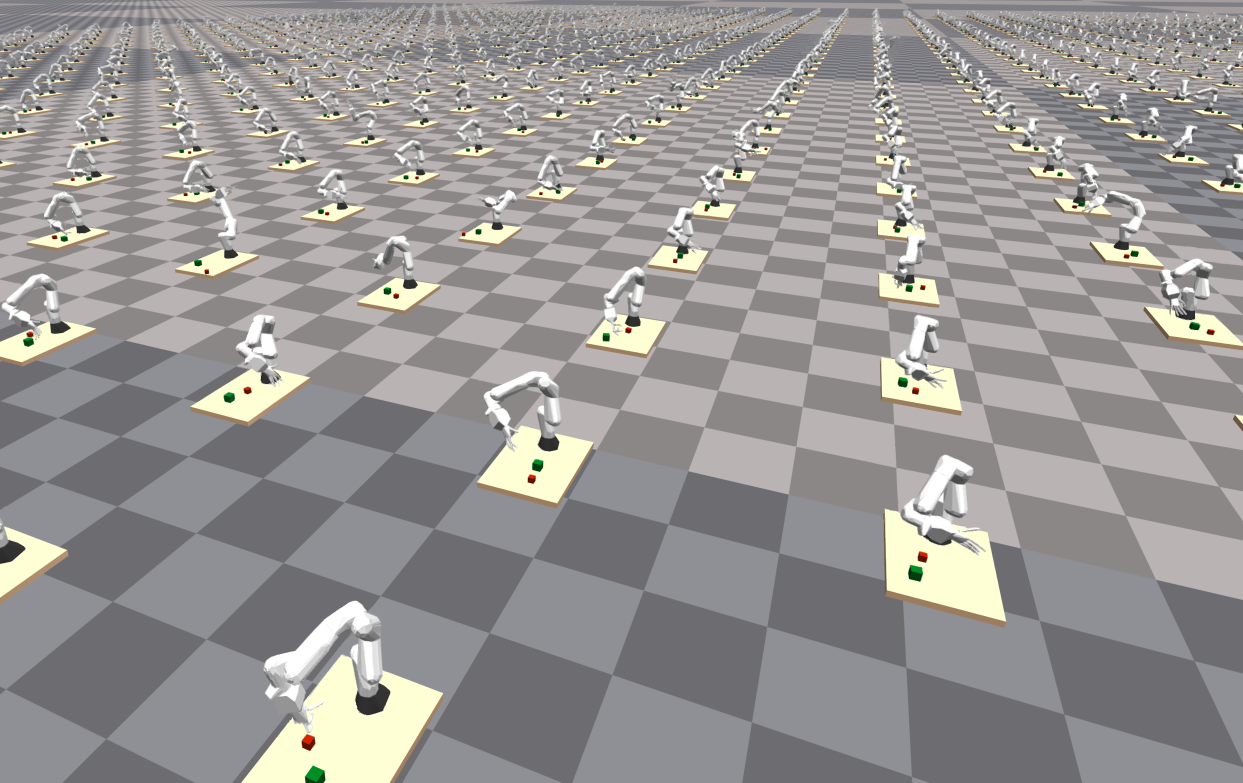
\includegraphics[scale=0.3]{images/summary.png}
    \caption{Faive Hand Proto2-version combined with Franka Emika Panda visualized inside the training environment in Isaac Gym.}
    \label{IG}
\end{figure}

\subsubsection{Rewards and observation space}
 The rewards and penalties reported in \textit{Table 1} are used to train the system in Isaac Gym. All of them are designed such that they are continuous and output values between $-1$ and $1$. Then, they are scaled by the respective weight. Only the reward corresponding to the correct stack of the cube is expressed as a boolean value. While the purpose of \textit{Action penalty}, \textit{Reference joint penalty}, \textit{Joint limits penalty}, and \textit{Drop penalty} is to increase the safety of the robot movements, the remaining rewards are designed in such a way that they drive the learning process of the robot. First, the robot minimizes the distance of the hand from the grabbing cube. Second, it lifts the cube while maintaining a proper palm orientation. Then, it minimizes the distance between the two cubes, and finally, it stacks them (see Figure \ref{sequence}).
In particular, the success condition, namely the correct stack of the cube, is achieved when three conditions are satisfied:
\begin{enumerate}
    \item the distance of the cubes' centers in the x-y plane is lower than a given threshold.
    \item the distance of the cubes along the z-axis is lower than a given threshold (see in more detail in Figure \ref{y_axis}).
    \item the distance of the hand from the grabbed cube center is bigger than a given threshold.
\end{enumerate}
\renewcommand{\arraystretch}{2.5}
% create a page with a single table in it in landscape, according to https://tex.stackexchange.com/questions/19017/how-to-place-a-table-on-a-new-page-with-landscape-orientation-without-clearing-t
\afterpage{%
\clearpage% Flush earlier floats (otherwise order might not be correct)
\thispagestyle{empty}% empty page style (?)
\begin{landscape}% Landscape page
\begin{table}[p]
\small
    \centering
    %\scriptsize
    \begin{tabular}{|c|c|c|c|}
    \hline \textbf{\textit{Reward}} & \textbf{\textit{Formula}} & \textbf{\textit{Weight}} & \textbf{\textit{Justification}}\\
    \hline Action penalty & $|| \bm a ||_2$ & -0.001 & Prevent large actions\\
    \hline Reference joint penalty & $|| \bm q_{arm} - \bm q_{start} ||_2$ & -0.1 & Prevent arm joints from moving from the reference position\\
    \hline Joint limits penalty & $|| \max(\bm 0, - \bm q_{min} - \bm q_{arm}, \bm q_{arm} - \bm q_{max} ||_2$ & -0.1 & Prevent arm joints to move beyond the joint limits \\
    \hline Drop penalty & $|| \bm p_{grab} - \bm p_{ref} ||_2 > \SI{50}{\cm}$ & -1.0 & Prevent cube to be dropped \\
    \hline Hand-cube distance & $ 1 - \tanh(10 \frac{|| \bm p_{grab} - \bm p_{hand} ||_2 + \sum_{n=1}^{5} || \bm p_{fingertip_{i}} - \bm p_{grab} ||_2}{6}) $ & 0.1 & Reward distance from the hand to the cube\\
    \hline Cube lifting & $ clip(0, \frac{\bm p_{z_{grab}} - \bm l_{grab}}{0.04}, 1)$ & 1.5 & Reward the lift of the cube\\
    \hline Palm orientation & $ \langle \hat{\bm j}_{palm}, \hat{\bm k}_{world} \rangle$ & 0.01 & Reward the palm for facing the table\\
    \hline Cube-cube distance & $|| \bm p_{grab} - \bm p_{ref} ||_2$ & 2.0 & Reward distance from the cubes\\
    \hline Correct stack & $ || \bm p_{xy_{grab}} - \bm p_{xy_{ref}} ||_2 < \SI{2}{\cm} \wedge || \bm p_{z_{grab}} - \bm p_{z_{ref}} ||_1 < \SI{2}{\cm} \wedge || \bm p_{hand} - \bm p_{grab} ||_2 > \SI{8}{\cm}$ & 400.0 & Reward the correct stack of the cube\\
    \hline
    \end{tabular}
    \caption*{\textit{Table 1}: Rewards and penalties used during training.}
\end{table} % better to report the formulas too? --> YES
\end{landscape}
}

\newpage
\begin{figure}[!hb]
    \centering
    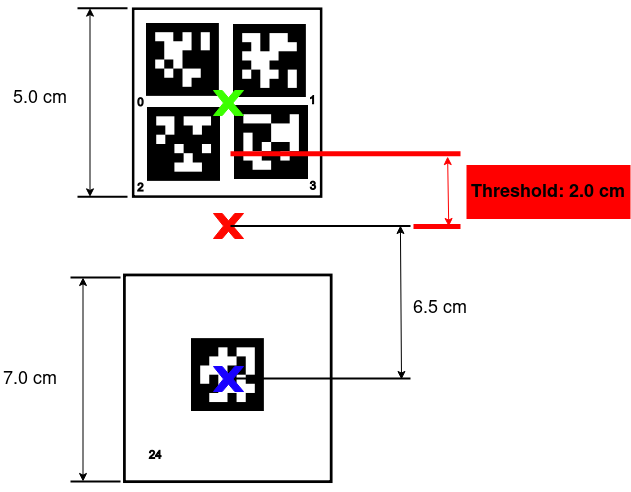
\includegraphics[scale=0.6]{images/markers_latex.png}
    \caption{Condition to stack the grabbing cube on the reference cube. The center of the grabbing cube (green) must be inside the red threshold.}
    \label{y_axis}
\end{figure}


\begin{figure}[!hb]
    \centering
    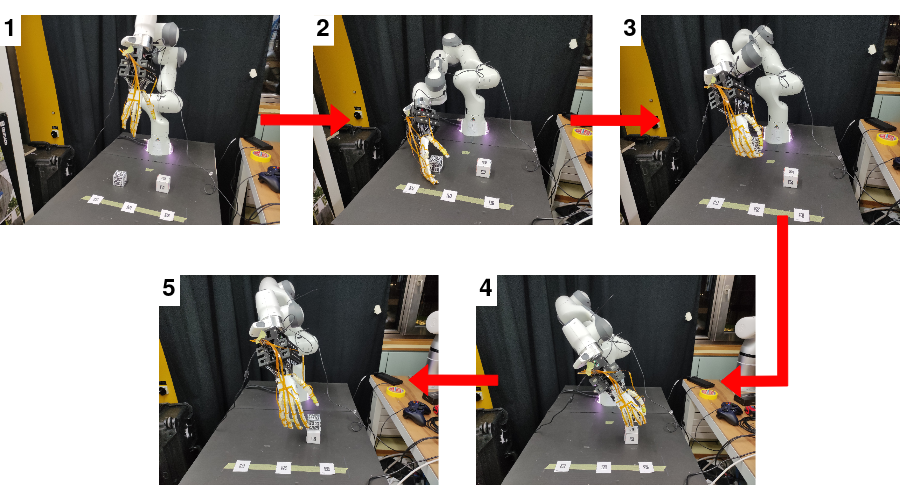
\includegraphics[scale=0.65]{images/movement_sequence.png}
    \caption{Sequence of pictures representing the expected behaviour of the robot. The robot has been manually moved to take the pictures.}
    \label{sequence}
\end{figure}

The same observations used by the actor and the critic networks are reported in \textit{Table 2}. The agent uses both proprioceptive and exteroceptive data, due to the need to know objects' position and orientation. As part of the implementation set-up, two cameras are used to estimate the pose of the cubes in the environment, and then generate proper commands for the robot to interact with the system. Therefore, the cubes are covered with markers to be detected by the vision system. It is important to notice that no measurements coming directly from the hand are used. This is useful because it is not possible to measure directly the hand joint angles, which are expressed as a non-linear mapping with the tendon length, and affected by noise due to slack in the tendons. Furthermore, Isaac Gym ignores the tendons-level information and considers the hand only as a joint-level robot. The hand joint angles used by $dof\_pos\_target$ and $actions$ are the output of the actor network in the simulation, and not a measurement coming directly from the hand, for example of the angles read by the motor encoders.

\begin{table}[h]
    \centering
    \begin{tabular}{|c|c|c|}
    \hline \textit{\textbf{Observations}} & \textit{\textbf{Dimension}} & \textit{\textbf{Description}}\\
    \hline obj\_pos & 3 & Cube position\\
    \hline obj\_quat & 4 & Cube quaternion\\
    \hline eef\_pos & 3 & End-effector position\\
    \hline eef\_quat & 4 & End-effector quaternion\\
    \hline hand\_to\_obj\_pos & 3 & Hand-cube relative position\\
    \hline obj\_to\_goal\_pos & 3 & Cubes relative position\\
    \hline dof\_position & 7 & Arm joint angles\\
    \hline dof\_pos\_target & 23 & Hand and arm joint angles\\
    \hline actions & 23 & Hand and arm joint commands\\
    \hline
    \end{tabular}
    \caption*{\textit{Table 2}: Observations used during training for the actor and critic networks in Isaac Gym.}
\end{table}

\newpage
\subsubsection{Action space}
Joint position control is adopted to command both the robotic arm and the biomimetic hand. The action $\textbf{a}$ expresses the relative change in the joint angle command. It is first clipped between $-1$ and $1$, then it increments the desired joint angle $\hat{\textbf{q}}$. Moreover, relative control is exploited, leading to (\ref{control_law}):

\begin{equation}
    \hat{\textbf{q}} = clip(\hat{\textbf{q}}+v_{max} \Delta t \textbf{a}, \textbf{q}_{min}, \textbf{q}_{max})
    \label{control_law}
\end{equation}

where $\Delta t$ is the timestep and $v_{max}$ is a constant scalar that caps the maximum speed of the joints from the policy. $v_{max}$ is set to $7 rad/s$. After the action updates the desired joint angle, it is clipped between the minimum $\textbf{q}_{min}$ and maximum $\textbf{q}_{max}$ joint angles of the robot hand.
This control law encourages policy exploration since the maximum speed is bigger than the one physically reachable by the robot and the hand, and mimics joint torque control by using the relative speed.

\subsubsection{Domain randomization}

To compensate for the inaccuracy of the physics engine, make the policy more robust, and close the sim-to-real gap, domain randomization is applied to some of the system's physical properties, namely the observations, and scale, mass and friction of the cube (see \textit{Table 3}). Domain randomization is not applied to the robotic arm's physical parameters (i.e. mass, friction, stiffness, and damping) because the robot is moved very slowly for safety reasons, and then the dynamic effects are neglected.

\begin{table}[h]
    \centering
    \begin{tabular}{|c|c|c|}
    \hline \textit{\textbf{Quantity}} & \textit{\textbf{Distribution}} \\
    \hline Observation noise & $\mathcal{N}(0;\;0.005) m$\\
    \hline Observations correlated noise & $\mathcal{N}(0;\;0.005) m$\\
    \hline Cube friction & $\mathcal{U}(0.7;\;1.3)$\\
    \hline Cube scaling & $\mathcal{U}(0.98;\;1.02)$\\
    \hline Cube mass & $\mathcal{U}(0.5;\;1.5)$\\
    \hline
    \end{tabular}
    \caption*{\textit{Table 3}: Quantities modified by using domain randomization and correspondent noise distribution.}
\end{table}
    
% A Gantt chart should be included in proposals. It demonstrates the planned timeline of the project.
% It is not necessary to create the chart with LaTeX like shown here. This is just an option to potentially save you some time.
%% http://www.ctan.org/pkg/pgfgantt

\begin{figure}[h!]
\begin{center}

\begin{ganttchart}[
x unit = 0.7cm,
y unit title=0.6cm,
y unit chart=0.6cm,
vgrid,
hgrid,
title label anchor/.style={below=-1.7ex},
title height=1,
bar/.style={fill=ETH-l-blue,
            draw=black,
            line width=0.5pt},
incomplete/.style={fill=white},
progress label text={},
bar height=0.7,
group left shift=0.0,
group right shift=0.0,
group top shift=0.5,
group height=0.2,
group peaks width=0.4,
group peaks height=0.25,
group peaks tip position=0,
milestone height=0.7,
milestone label anchor/.style={ below left=-1.7ex and 0.2ex}
]{1}{16}

% Labels
\gantttitle{Semester Thesis Timeline}{16} \\
\gantttitlelist{"September"}{4} \gantttitlelist{"October"}{5} \gantttitlelist{"November"}{4} \gantttitlelist{"December"}{3} \\
\gantttitle{Week of the Year}{16} \\
\gantttitlelist{36, ..., 51}{1} \\

% Group 1
\ganttgroup{Simulation}{1}{16}\\
\ganttbar{Literature search}{1}{5} \\
\ganttbar{Mujoco}{4}{6} \\
\ganttbar{Isaac Gym}{4}{16}\\
\ganttmilestone{Proposal Presentation}{8} \\

% Group 2
\ganttnewline
\ganttgroup{Implementation}{10}{16} \\
\ganttbar{Set-up}{10}{10} \\
\ganttbar{Tests}{11}{16} \\
\ganttbar{Documentation}{15}{16} \\
\ganttmilestone{Final Presentation}{15}


% Relations
%\ganttlink{elem3}{elem7}

\end{ganttchart}
\end{center}
\caption{Gantt Chart of the proposed Semester Thesis}
\label{fig:Gantt Chart}
\end{figure}


\subsection{Training results}
The results of the training are collected using Weights and Biases. Thanks to this tool, it is possible to visualize the performances of the agent. In particular, three quantities are used to evaluate the success of the policy:
\begin{enumerate}
    \item the distance between the cubes' centers in the x-y plane. The success is achieved if it is lower than 0.02 meters.
    \item the distance of the cubes along the z-axis. The success is achieved if it is lower than 0.02 meters (see Figure \ref{y_axis}).
    \item the distance of the hand from the center of the grabbed cube. The success is achieved if it is greater than 0.08 meters.
\end{enumerate}

% plots of the policies
It is possible to visualize four quantities, useful to evaluate several policies' performances:
\begin{enumerate}
    \item success reward: evolution of the success reward during the training.
    \item success rate: percentage of instances achieving success at the end of each episode.
    \item total reward: total reward achieved during the training.
    \item episode length: time until which the reset condition is triggered in each episode. The reset condition is achieved either if it succeeds, if the cube is dropped from the scene, or if the maximum episode length is achieved.
\end{enumerate}

The results are visualized by taking the mean of the five runs with different random seeds. Three different observation noise variance realizations are considered, as shown in the legend. An area of $\pm\sigma$ is shown around the curves.

% plots go here
%%% If I want to add some comments to the plots, should I write them in the caption or under the figure?  Answer: inside caption
\newpage
\begin{figure}[!hb]
    \centering
    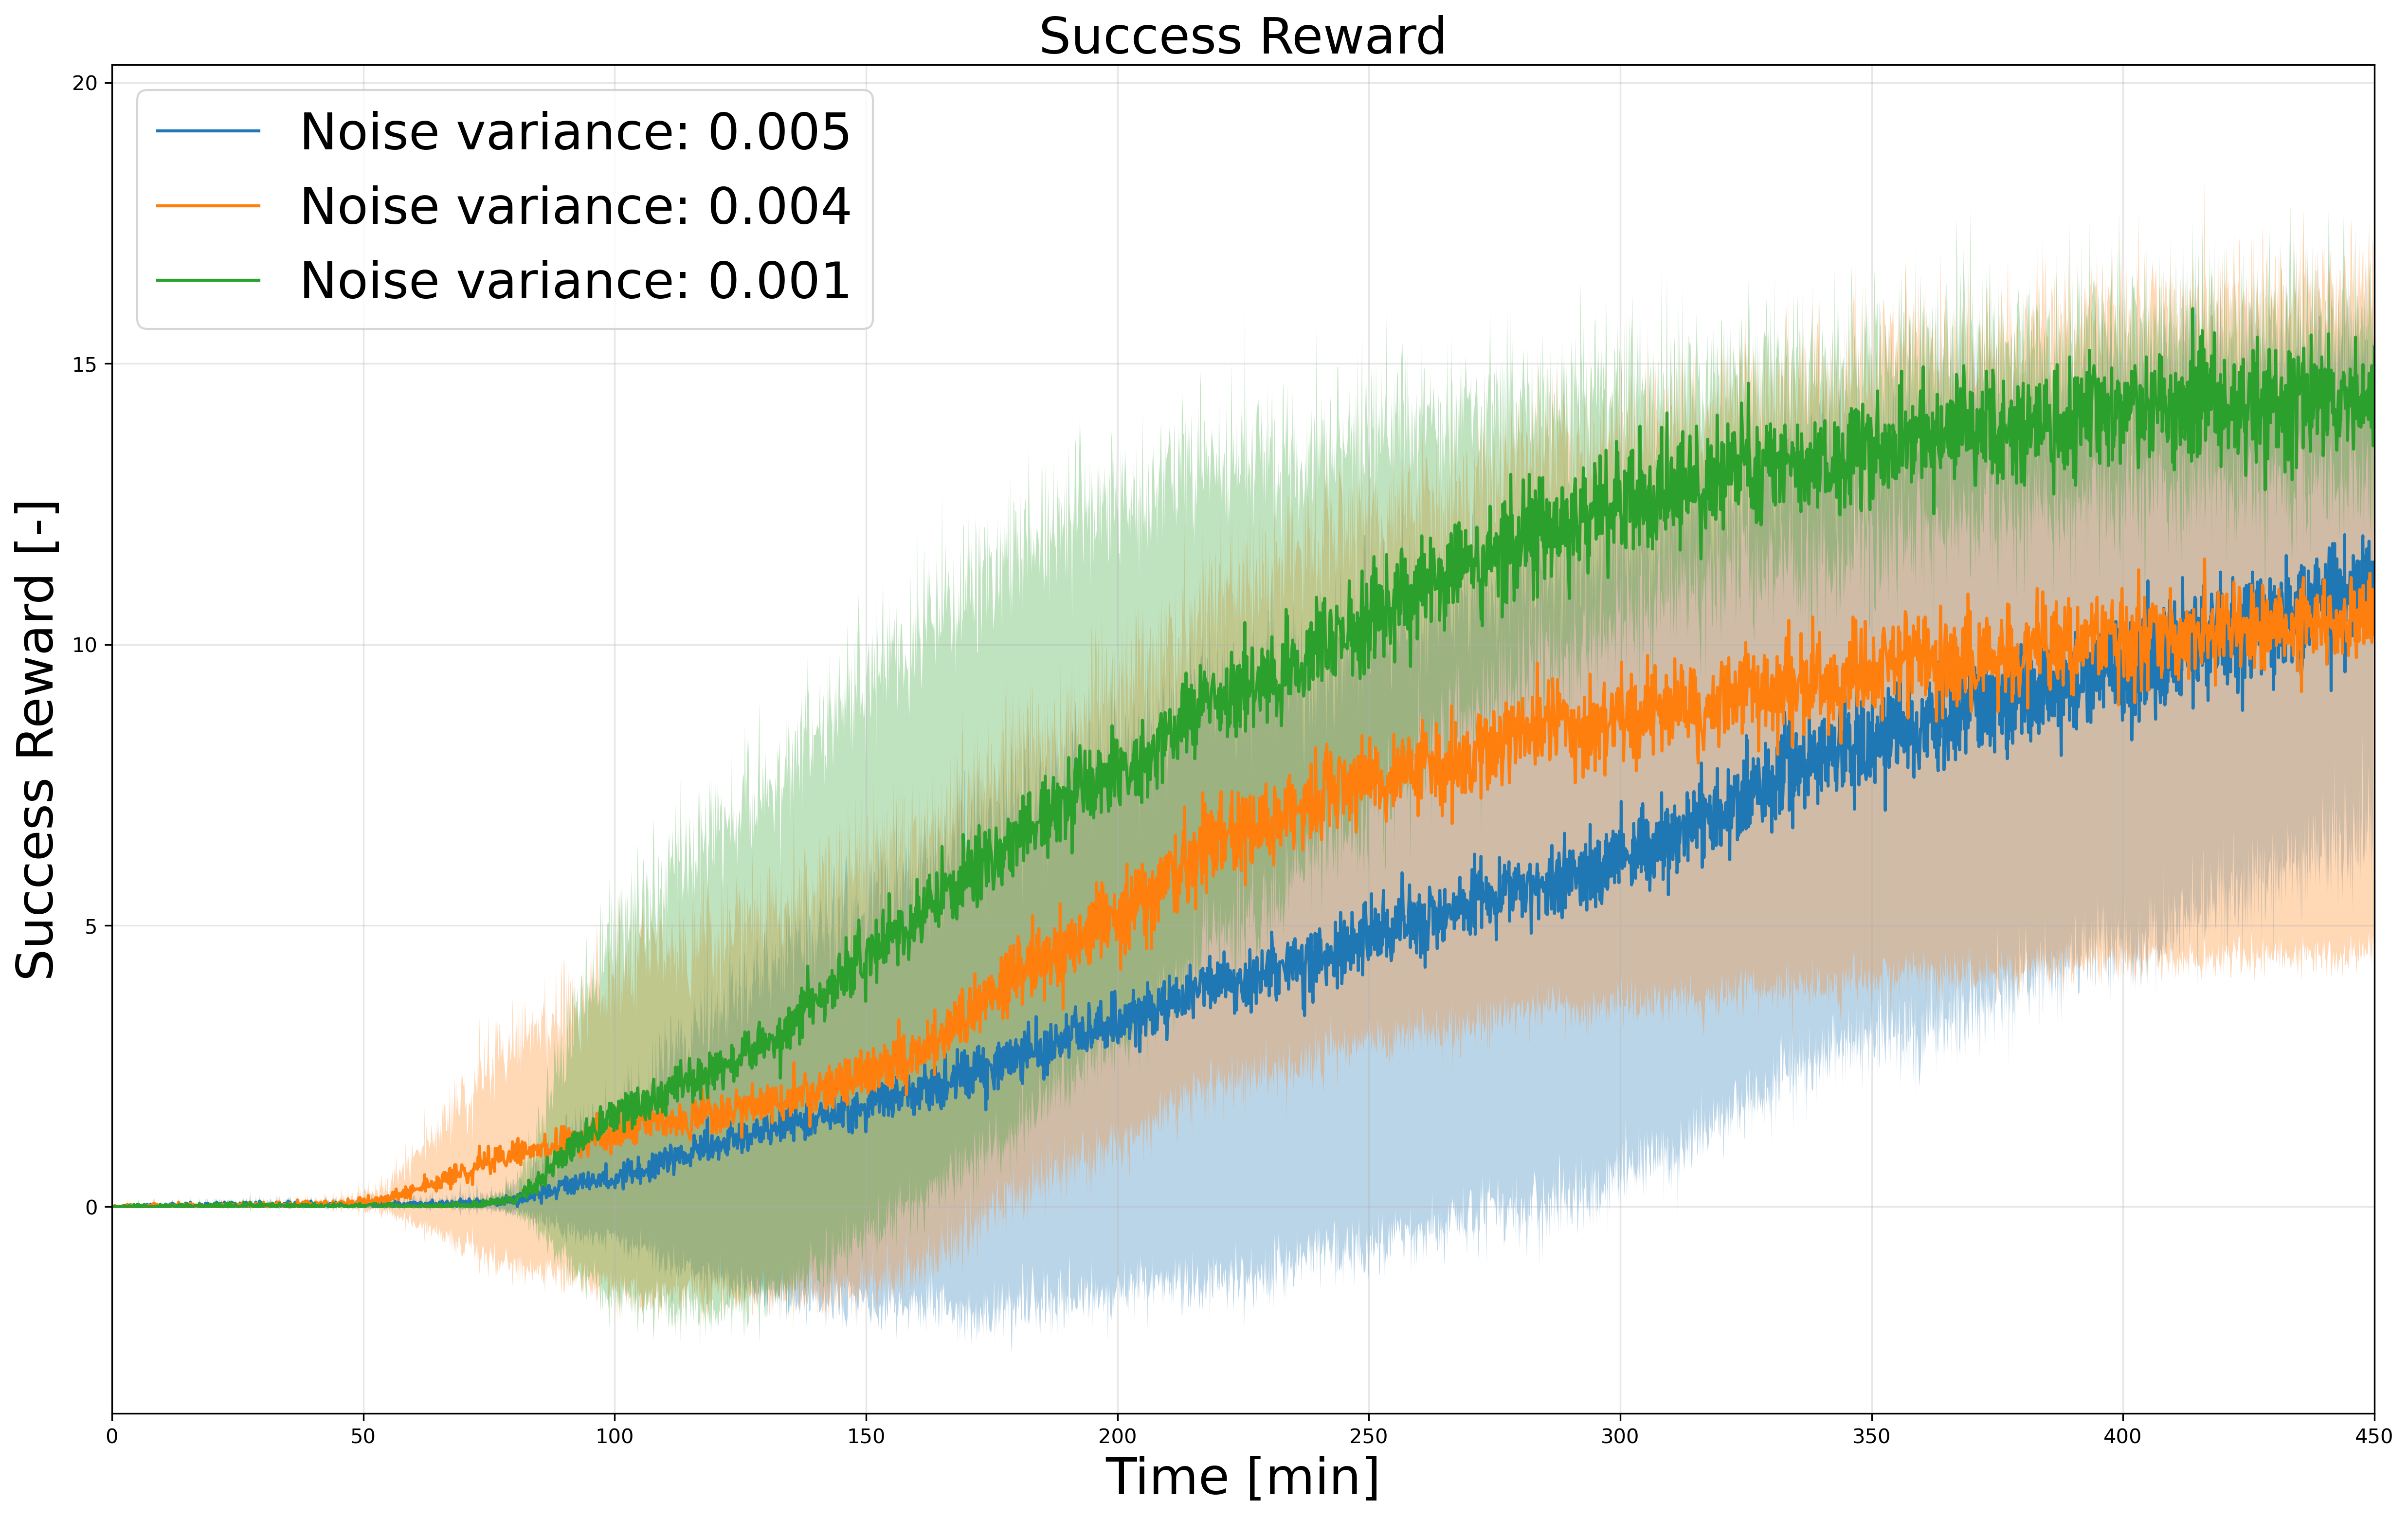
\includegraphics[scale=0.3]{images/Success Rewardv3.png}
    \caption{Success reward. It is increasing until the agent finds a policy to succeed in the task. Then, it converges.}
\end{figure}

\vspace{2cm}

\begin{figure}[!hb]
    \centering
    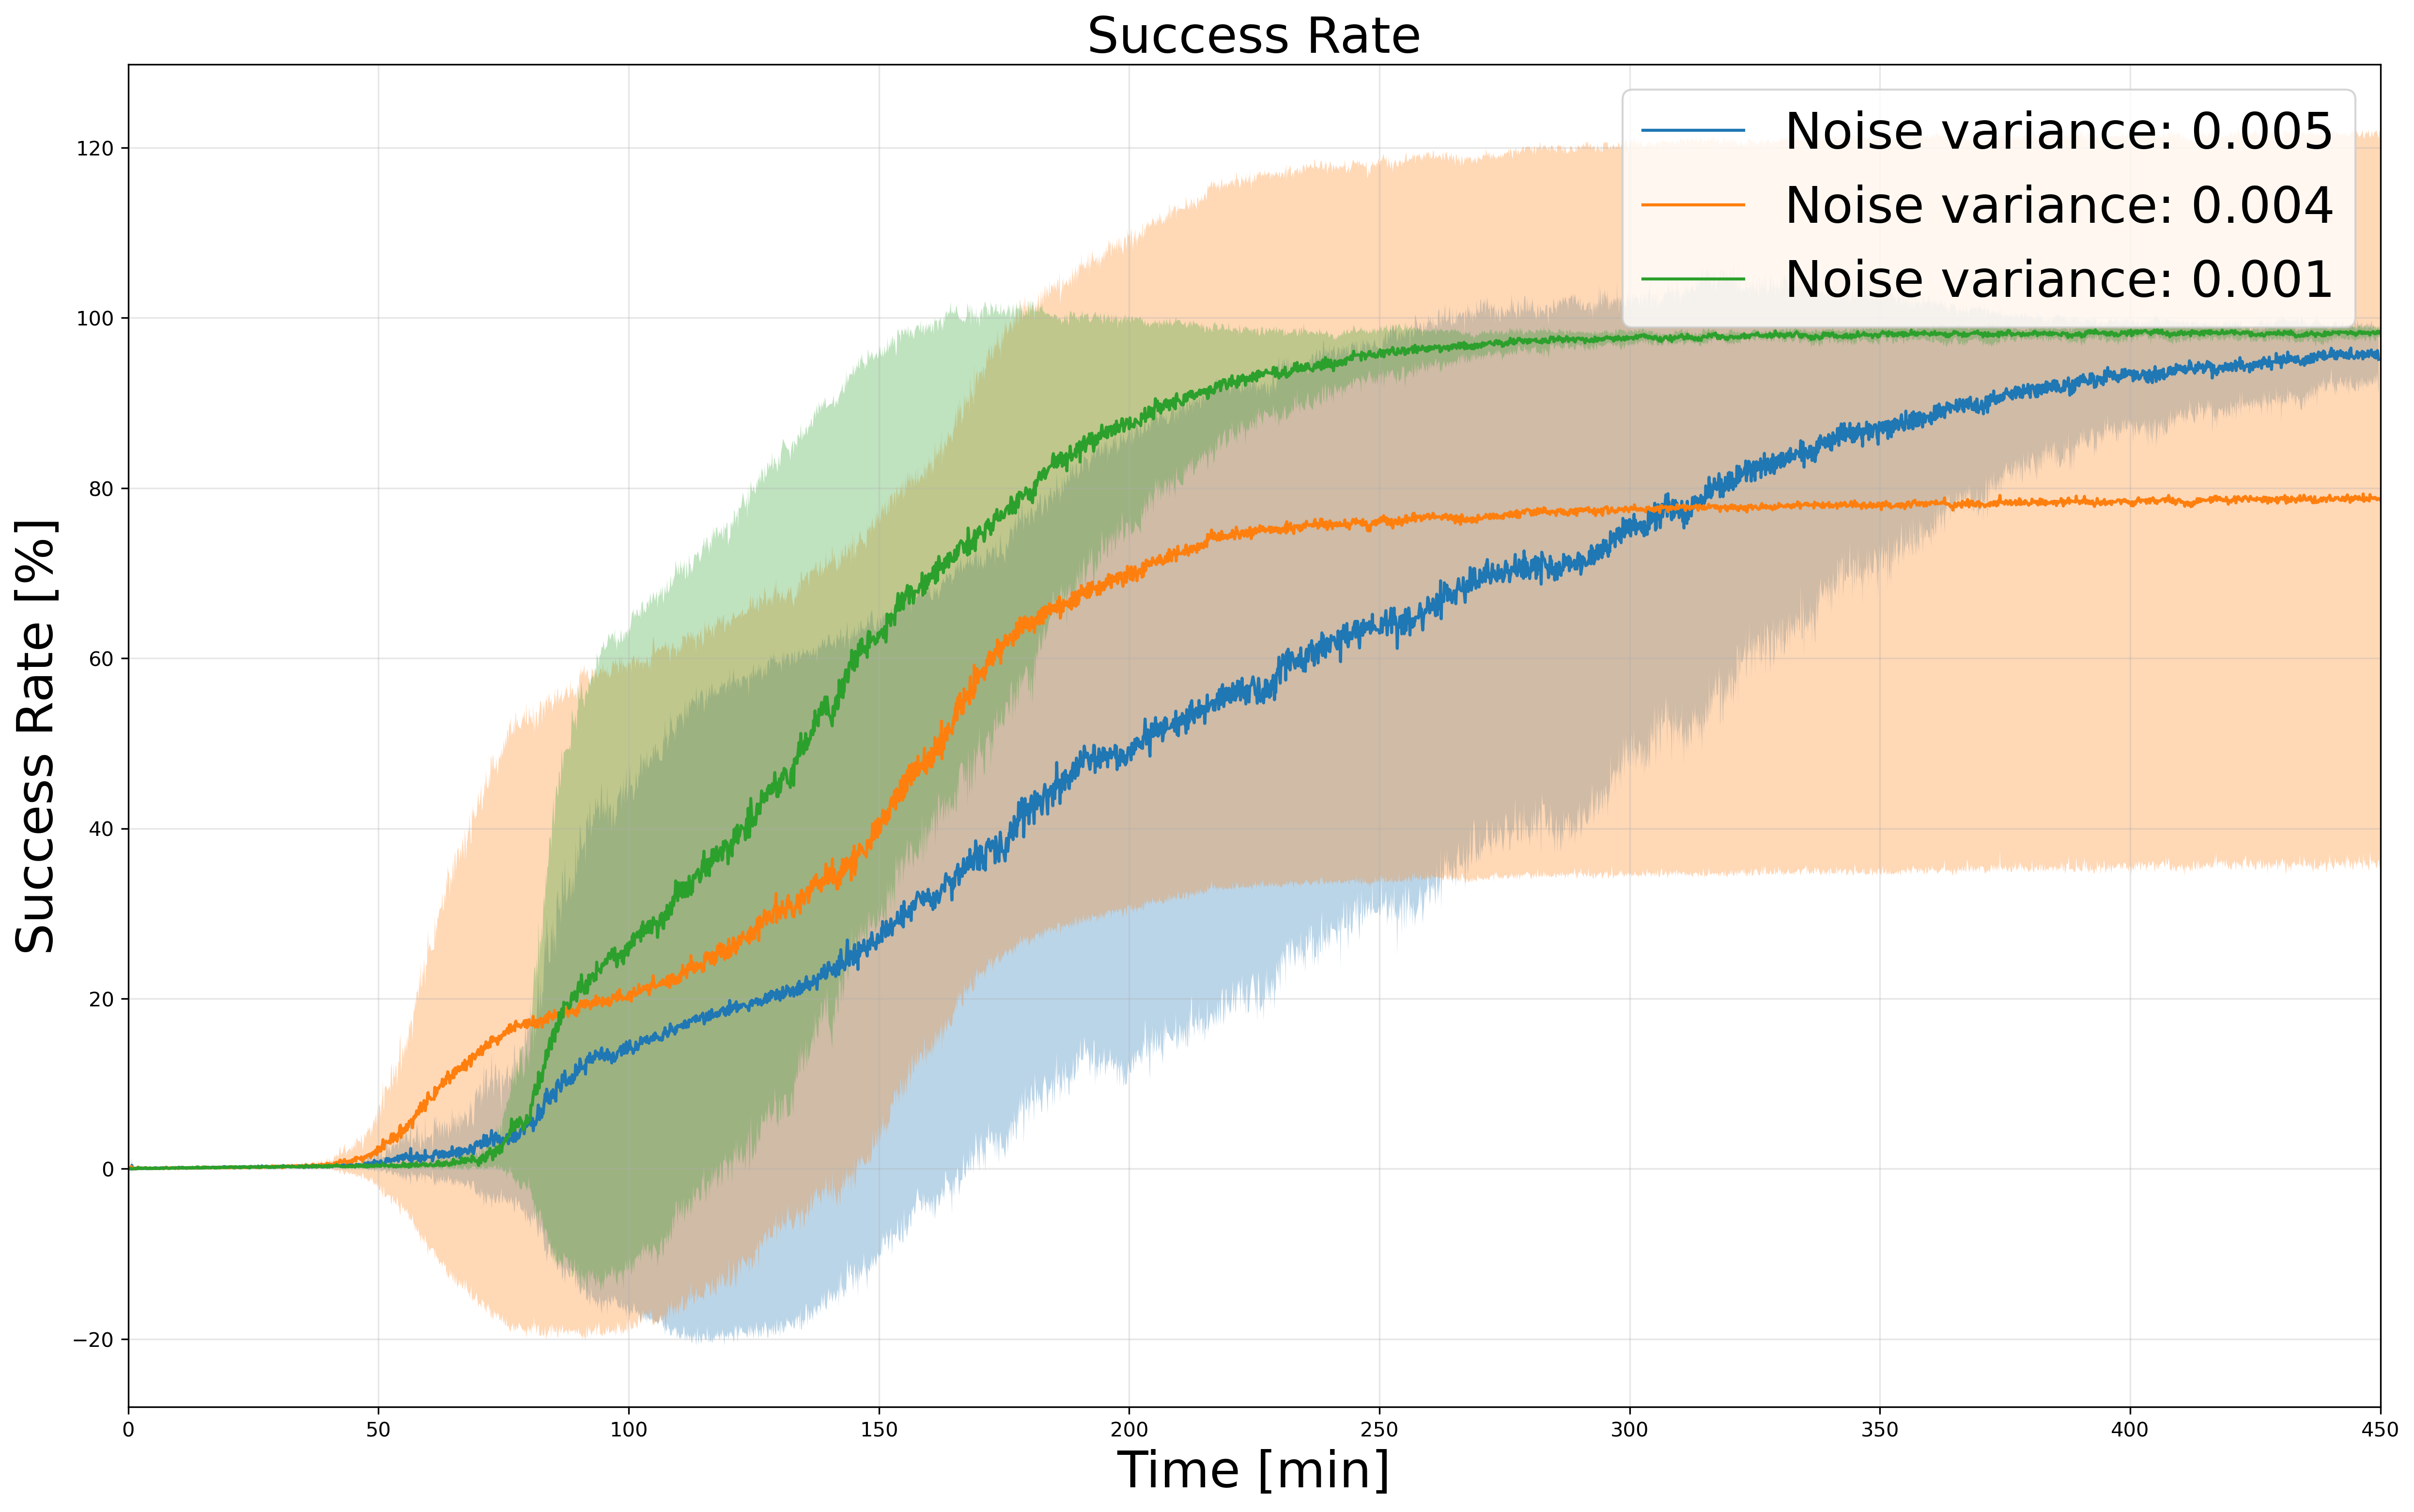
\includegraphics[scale=0.3]{images/Success Ratev3.png}
    \caption{Success rate. When the noise variance is 0.004, one out of 5 experiments does not succeed, reducing the overall success rate. The negative success rate is due to the high standard deviation, originating from the different learning times of the different seeds.}
\end{figure}

\newpage

\begin{figure}[!hb]
    \centering
    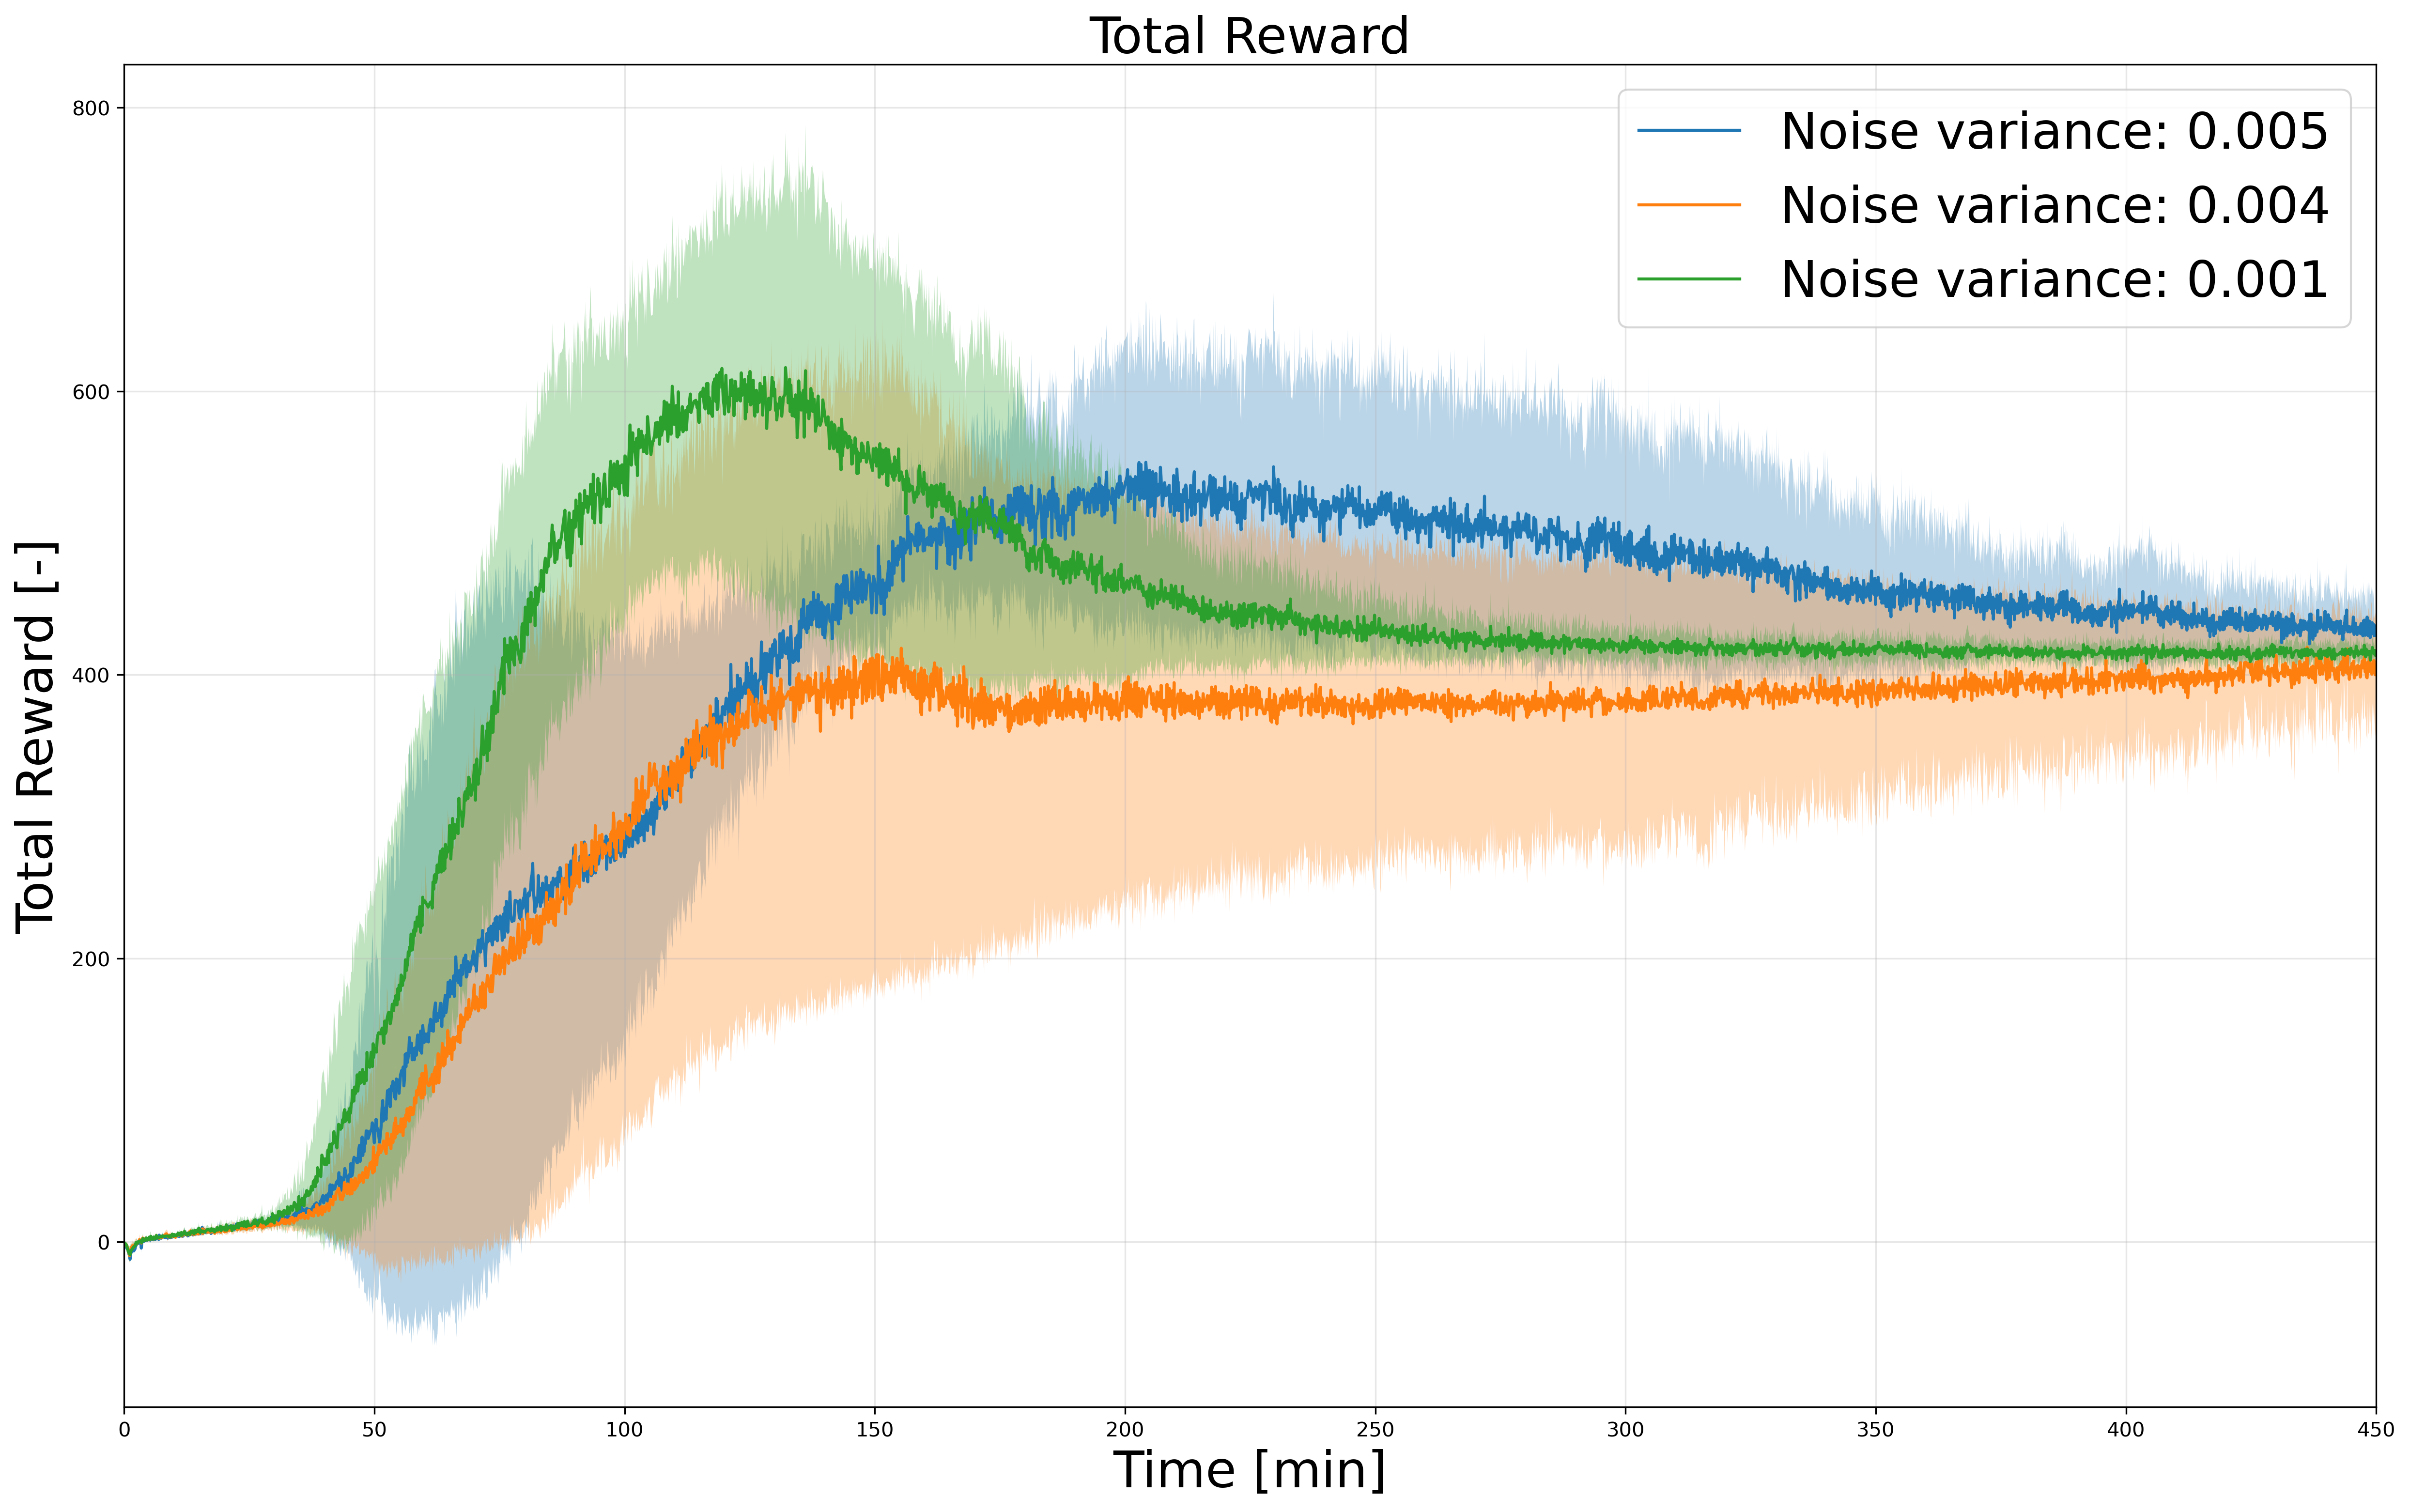
\includegraphics[scale=0.3]{images/Total Rewardv3.png}
    \caption{Total reward. It is increasing until the agent finds a policy to succeed in the task. Then, it converges.}
\end{figure}

\vspace{2cm}

\begin{figure}[!hb]
    \centering
    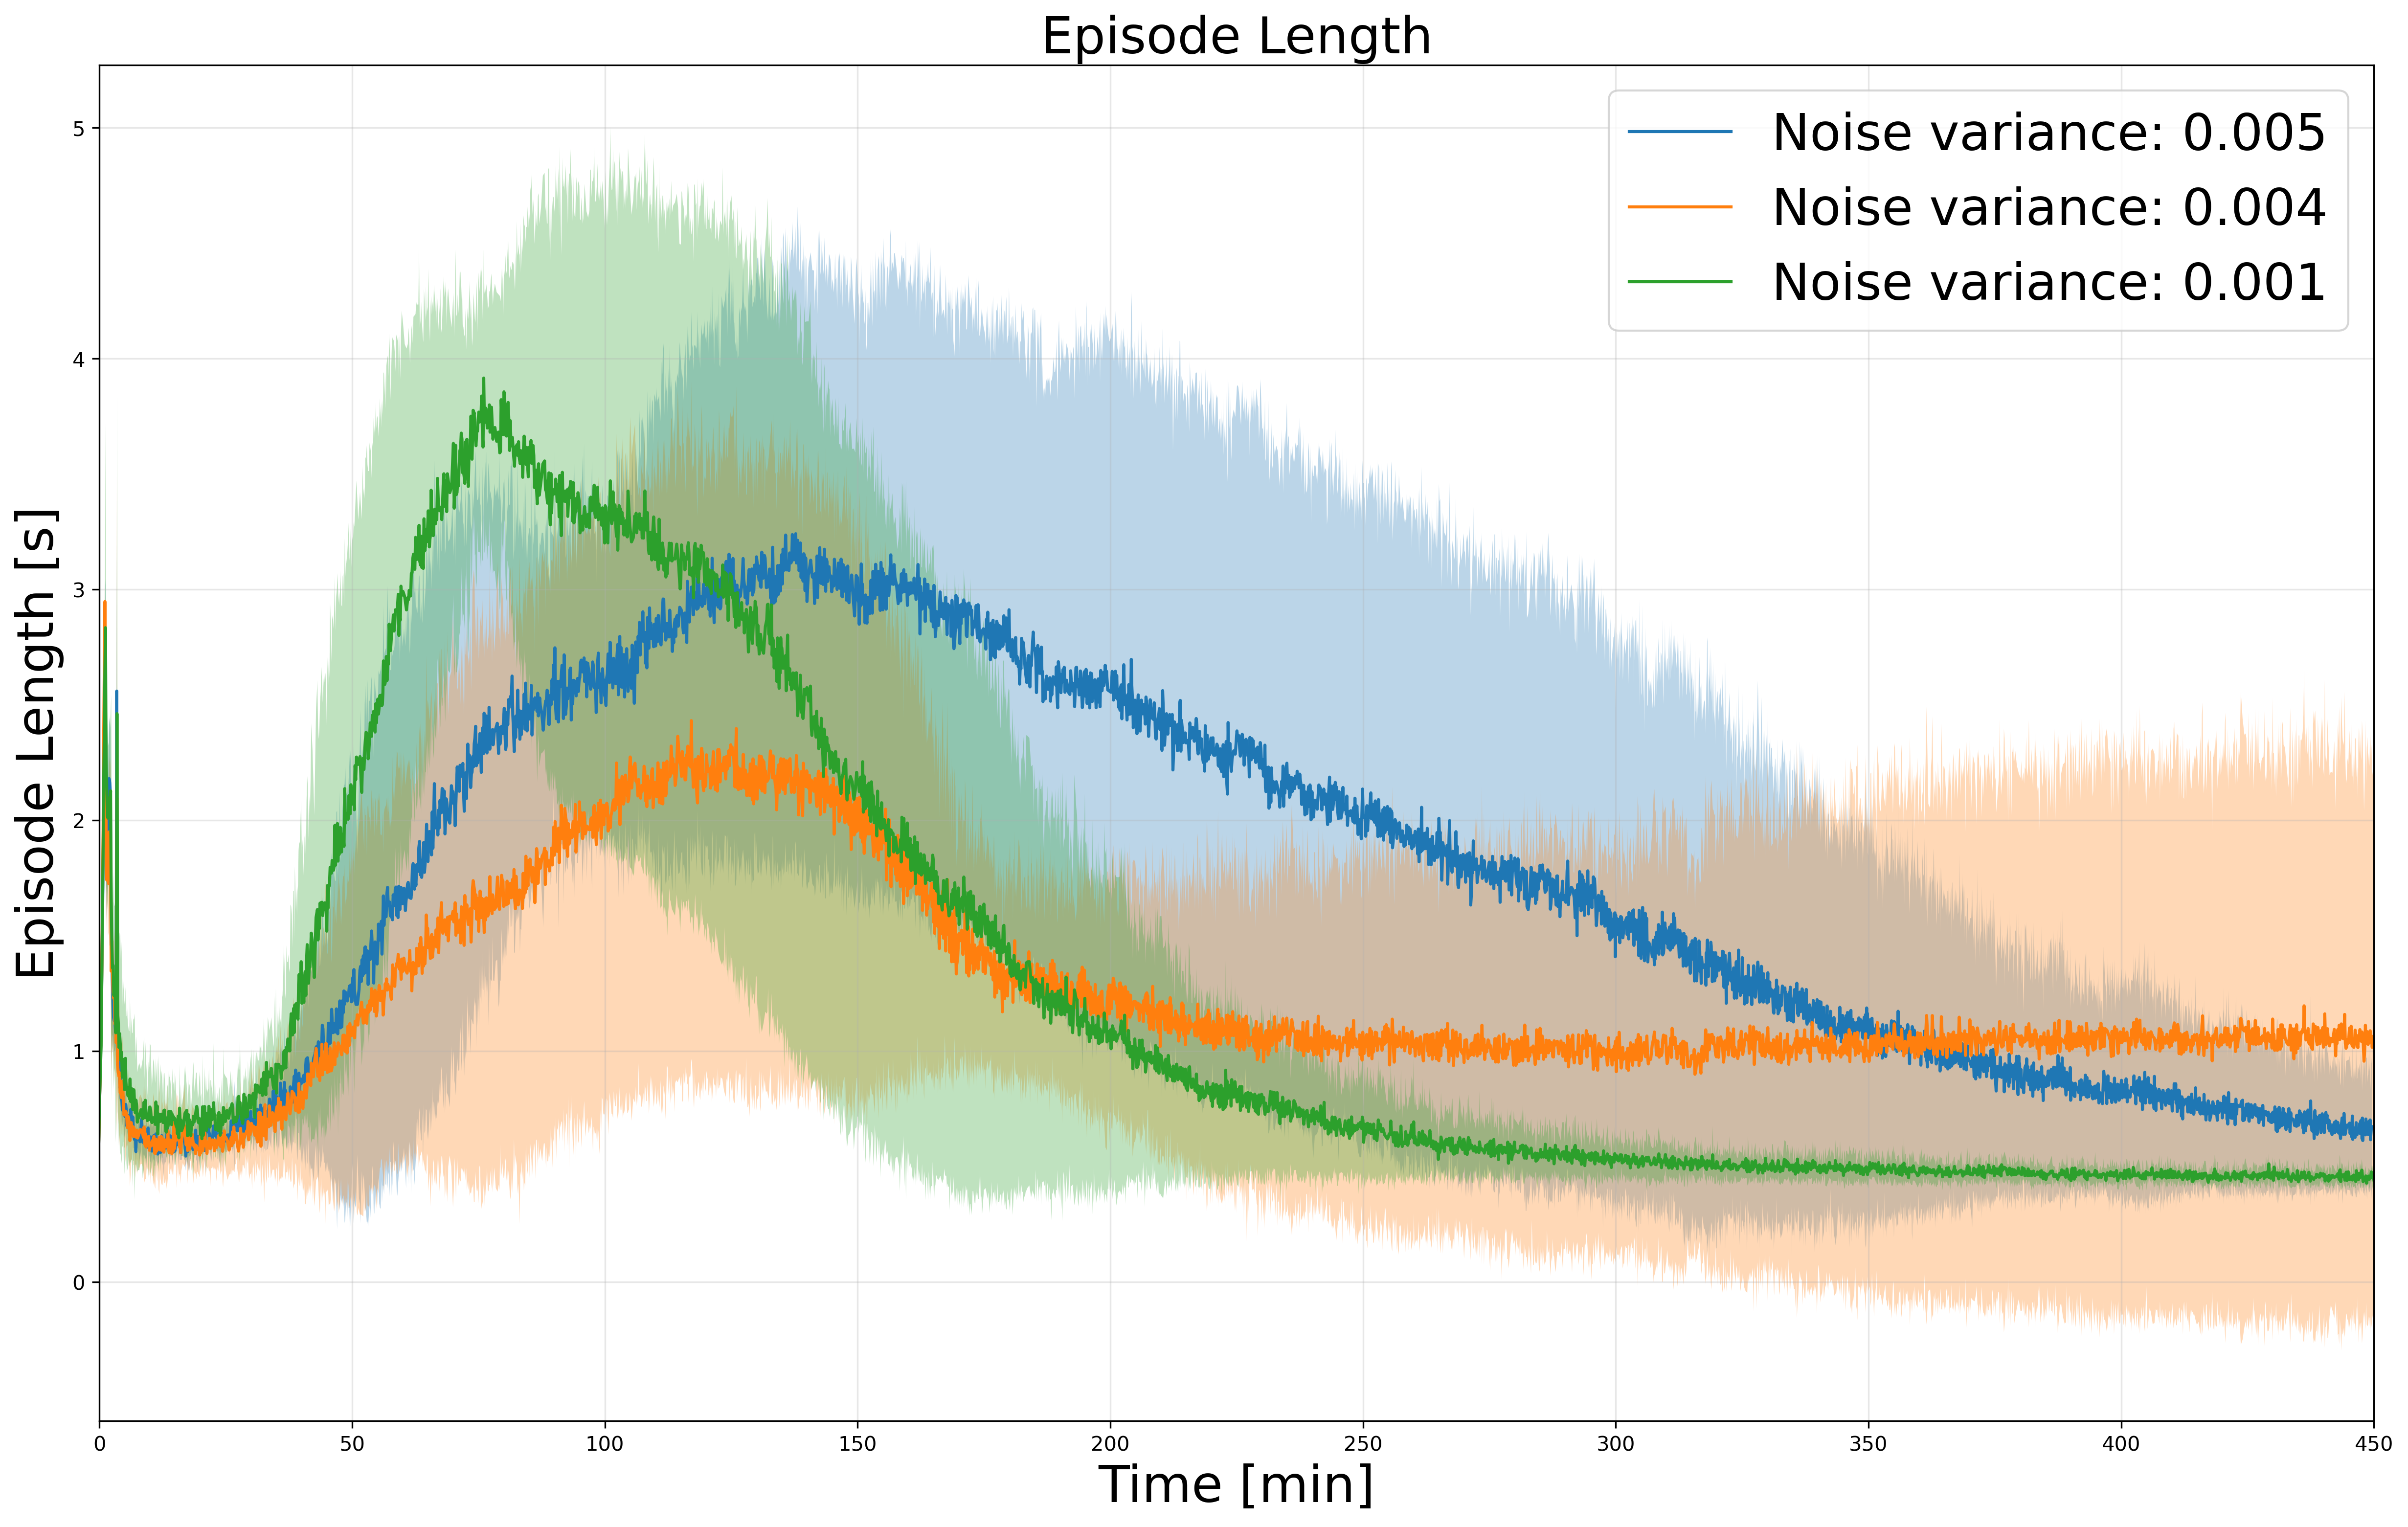
\includegraphics[scale=0.3]{images/Episode Lengthv3.png}
    \caption{Episode length. It has three distinct phases. At the beginning, the average episode length is decreasing, because the agent is failing in grabbing the cube, and then, the training is constantly resetting since it triggers the reset condition. As time increases, the agent learns what is the proper way to grab, hold, and move the cube. Then, the average episode length increases. Finally, when the agent finds what is the proper policy to accomplish the task, the episode length starts decreasing as the optimization goes on.}
\end{figure}

\newpage

\subsection{Experiment setup}
After training is finished, the neural network of the actor is exported to an ONNX format and run on the robot. For the implementation of the policy on a real-world set-up, ROS 1 Noetic has been used. A brief description of the hardware and software components is presented with more details in the following subsections.

\subsubsection{Hardware architecture}
In terms of hardware, there is the main robot set-up: the Faive Hand Proto2 and a Franka Emika Panda arm. There are three computers, all connected via Ethernet:

\begin{enumerate}
    \item Franka Emika Control computer: handles low-level control of the robotic arm.
    \item Intel NUC: runs ROS master, handles higher-level control of the robotic arm.
    \item Desktop workstation: runs top-level tasks (cube poses tracking, logging, high-level control).
\end{enumerate}

%% figure with the hardware
\begin{figure}[!hb]
    \centering
    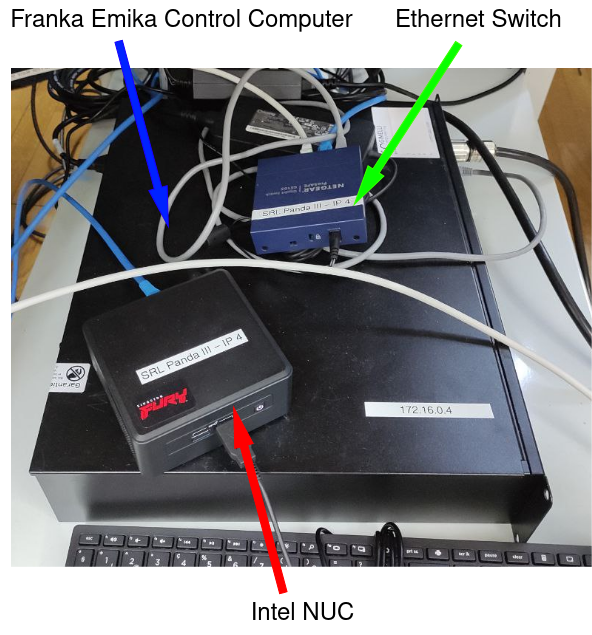
\includegraphics[scale=0.8]{images/hardware_steup.png}
    \caption{Hardware architecture.}
\end{figure}

Furthermore, two OAK-D Pro cameras\footnote{\url{https://shop.luxonis.com/products/oak-d-pro?variant=42455252369631}} have been used (see Figure \ref{camera}). The cube poses are estimated using AprilTag markers\footnote{\url{https://github.com/AprilRobotics/apriltag}}. The first cube has one marker for each side, while the second one, which is the one supposed to be grabbed, has four markers for each side (see Figure \ref{markers}). The reason behind this choice is to avoid possible markers' occlusions that may happen when the hand is grabbing the cube. In this way, there are more markers available to obtain the cube pose. 
The estimated positions and orientations are expressed with respect to the center of the table, which is identified by placing three markers on its surface to ensure at least one of them is always visible.

\begin{figure}[!hb]
    \centering
    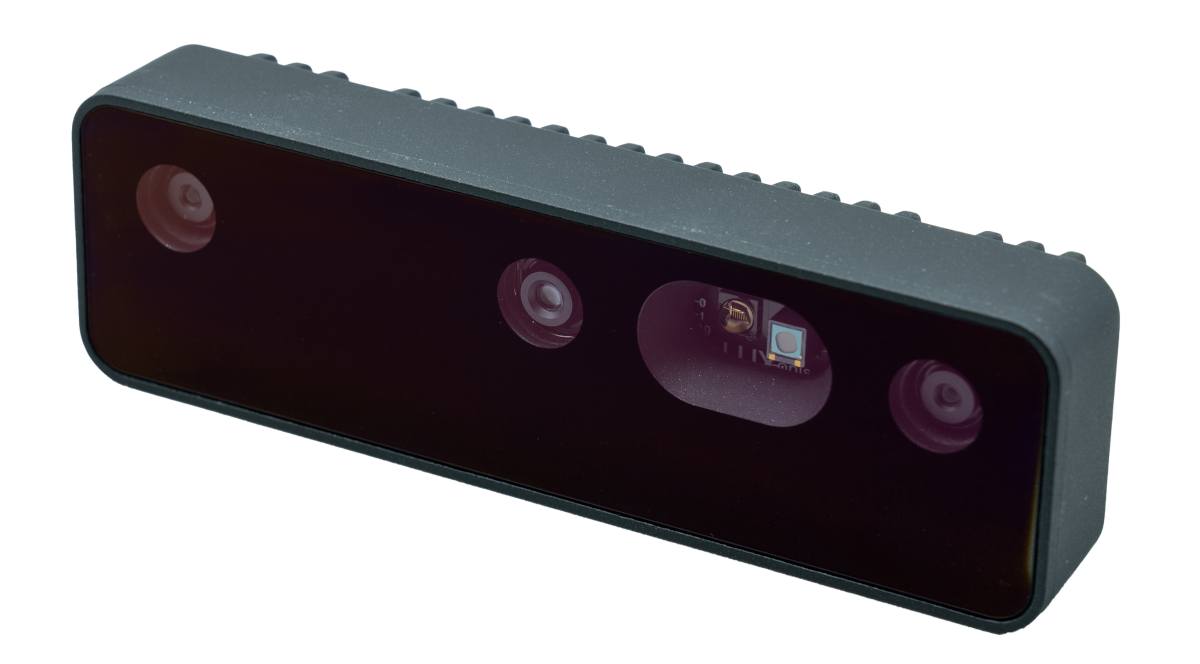
\includegraphics[scale=0.2]{images/oak-d-pro1.png}
    \caption{OAK-D Pro Camera.}
    \label{camera}
\end{figure}

\begin{figure}[!hb]
    \centering
    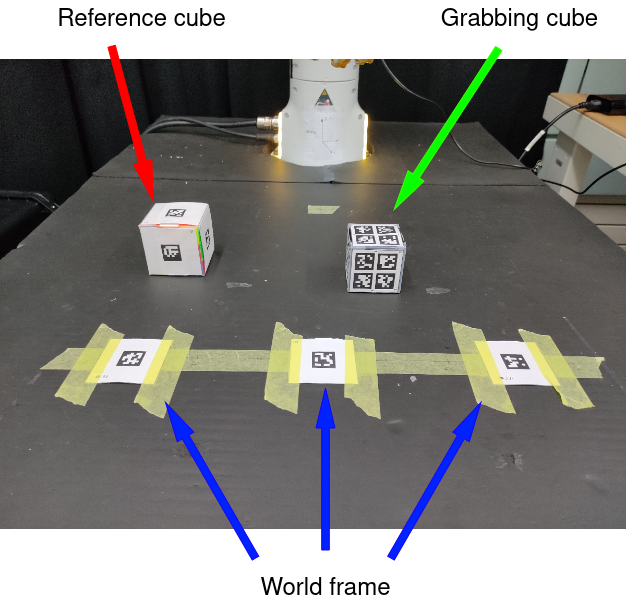
\includegraphics[scale=0.75]{images/markers (1).png}
    \caption{Objects covered with AprilTag Markers.}
    \label{markers}
\end{figure}

\newpage

\subsubsection{Software architecture}
The software system is built around ROS Noetic and written in Python. It is structured into two main distinct blocks:

\begin{enumerate}
    \item \textbf{pose tracking}: houses the ROS topic which publishes the messages representing the estimates of the cube poses. By using Apriltag markers, the algorithm detects the position and orientation of the objects in the scene and expresses their position directly with respect to the world frame. The markers are identified by a number that relates them to a specific object. Then, more markers identify one cube. So, it is necessary to average the poses coming from different markers to obtain the final cube poses. The data coming from the two cameras are averaged. In this way, if there are occlusions in only one of the cameras, the algorithm is still able to estimate the pose from the data coming from the other camera.
    \item \textbf{control policy}: houses the ROS topic which publishes the messages containing the control commands to the robotic arm and the Faive Hand. The control policy is inferred based on the observations read from the ROS messages, i.e. joint arm angles, joint hand angles, end-effector pose, and cubes poses. The relative control speed of the robot is slowed down with respect to the one used during training to avoid crashing into the table and breaking the hand.
\end{enumerate}
%%%%%%%%%%%%%%%%%%
% draw.io scheme %
%%%%%%%%%%%%%%%%%%
\begin{figure}[!hb]
    \centering
    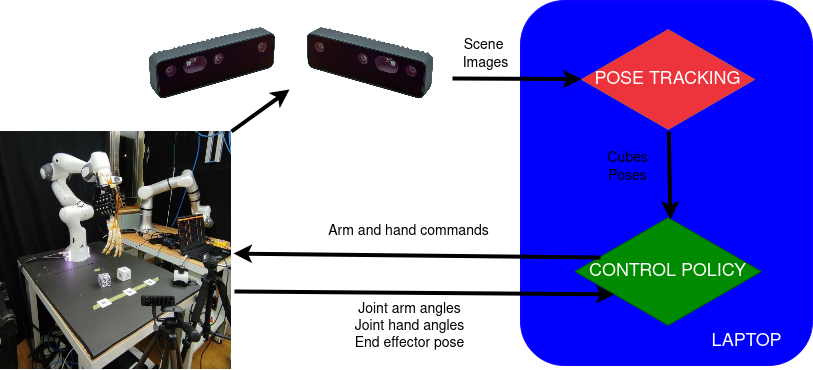
\includegraphics[scale=0.75]{images/control_structure_latex.png}
    \caption{Control flow diagram.}
\end{figure}

\subsection{Experiments results}
Several experiments have been run to evaluate the performances of the agent in a real-world environment. All the policies that were achieving success have been tested on the real robot. Several issues were encountered, in particular, related to the motion constraints that are acting on the robot to guarantee a safe movement of the robot with respect to itself and its surroundings (see Figure \ref{exps}). More in detail, three major constraints are limiting the robot's movement:
\begin{enumerate}
    \item self-collision avoidance, i.e. avoiding collision within the links of the robot.
    \item bounding-box, i.e. limiting the robot's workspace by manually defining limits within it. In particular, the constraints are expressed with respect to the end-effector position. 
    \item environment-collision avoidance, i.e. avoiding collision with the table.
\end{enumerate}
These elements were not considered during the training of the agent in Isaac Gym, and then, deeply affected the final policy (see Figure \ref{collisions}). 

\newpage

\begin{figure}[!hb]
    \centering
    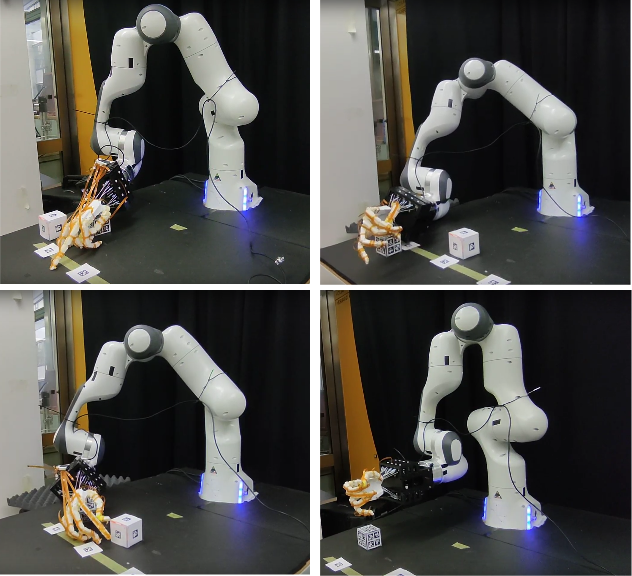
\includegraphics[scale=0.9]{images/experiments.png}
    \caption{Pictures of the robot blocked due to collisions while running different policies.}
    \label{exps}
\end{figure}

\vspace{1cm}

\begin{figure}[!hb]
    \centering
    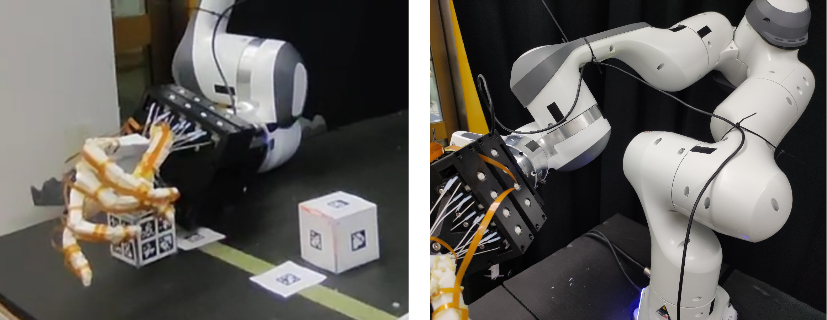
\includegraphics[scale=0.7]{images/collisions.png}
    \caption{Detailed pictures of the robot blocked due to collisions. In the left image, the robotic arm is touching the table, while in the right image, two links of the robotic arm are too close to each other.}
    \label{collisions}
\end{figure}

\newpage

% summary: what is working and what is not
As it is possible to see in the previous sections, the trainings are achieving a high success rate and promising performances. Nevertheless, the experiments performed in the laboratory showed that improvements are needed to transfer the learned policy to the real world.
On one hand, considering the whole experimental setup, several blocks are separately working (see Figure \ref{working}):
\begin{enumerate}
    \item the hand approaches the correct cube, i.e. the one which the agent is trained to grab.
    \item the hand holds the cube when it is manually placed in its proximity.
    \item following from the two previous achievements, the cube tracking algorithm is properly detecting the cubes' poses.
\end{enumerate}

\vspace{0.5cm}
\begin{figure}[!hb]
    \centering
    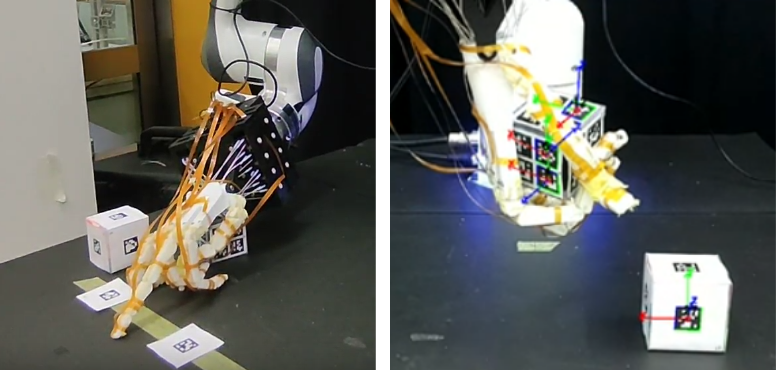
\includegraphics[scale=0.75]{images/working.png}
    \caption{Detailed pictures of the robot. In the left image, the robotic arm is getting closer to the grabbing cube, while in the right image, the hand is holding the grabbing cube.}
    \label{working}
\end{figure}
\vspace{0.5cm}

On the other hand, several components are not working correctly:
\begin{enumerate}
    \item the arm is colliding with itself and with the environment.
    \item the hand is not grabbing the cube after reaching it.
    \item the cubes are not stacked at the end, which was the desired goal.
\end{enumerate}

\newpage

\section{Conclusion}
This section describes the overall results of this Semester's Thesis, and identifies future improvements that are worth implementing.

\subsection{Overall results}
The training performed in Isaac Gym achieves consistent and relevant results. In particular, even if different seeds and noise realizations are used, the performances are satisfying. More in detail, the success rate and the episode length are very promising, since at least $80\%$ of the instances are completing the task in less than one second. These suggest that transferring the policies to the real world should be possible, but challenging as it is in many other applications.\\
Nevertheless, the experiments showed that there are still several elements to fix before closing the sim-to-real gap. Even if some of the components of the control pipeline are working separately, for example, the tracking of the position and orientation of the cubes, others are not behaving as expected. In particular, several constraints on the robot's movements were not taken into account when setting up the simulation environment, causing major problems when testing the policies in the real world.

\subsection{Future work}
Transferring the policy learnt in simulation to the real world is the main challenge of this Semester Thesis. When moving from simulation to reality, many issues are encountered, for example, dealing with the inherent noise that affects every measurement, or avoiding breaking the hardware.
Several improvements are possible for the current setup:
\begin{enumerate}
    \item considering the current design of the Faive Hand Proto2, since no measurements coming directly from the hand are used as observations for the reinforcement learning training, no additional sensors are needed. At the same time, covering the fingertips with silicone may make it easier to grasp the cubes, or other objects used in other applications.
    \item introducing explicitly the constraints on the robots, for example, the self collisions or the collision with the table, as penalties in the simulation, otherwise the robot will always stop when running the policy. This issue may be solved by designing custom penalties for the robot's joint positions with respect to their surroundings.
    \item the train in Isaac Gym lasts 4000 epochs. Completing one full training took, according to Weights \& Biases, more than 8 hours. Considering that the training in \cite{toshimitsu2023getting} used the same number of epochs, but the training lasted only a couple of hours, some improvements on the simulation are needed. In particular, the biggest computational effort should be in generating the video frames on Weights \& Biases used to visually evaluate the policy.
    \item improves the cubes detection algorithm, since the markers may get occluded and the measurements are affected by high noise. Different marker sizes can be exploited, and different placements of the cameras should be considered.
    \item introduces domain randomization on more elements, for example, the dynamical parameters of the robotics arm, or the actions. These additional elements might alleviate the difficulties in transferring the policy into the real world.
    
\end{enumerate}

\newpage

\printbibliography

%%%%%%%%%%%%%%%%%%%%%%%%%%%%%%%%%%%%%%%%%%%%%%%%%%%%%%%%%%%%%%%%%
%                        Document End                           %
%%%%%%%%%%%%%%%%%%%%%%%%%%%%%%%%%%%%%%%%%%%%%%%%%%%%%%%%%%%%%%%%%

\end{document}